\documentclass[a4paper,11pt]{article}
\usepackage[a4paper,tmargin={3cm},bmargin = {3cm}, lmargin={2cm}, rmargin={2cm}]{geometry} %Legt Format d. Dokuments fest
\usepackage{amsmath,array,hyperref,fancyhdr,amssymb,relsize,amsthm,answers,setspace,graphicx,color,tikz,lmodern,ngerman,geometry,titletoc,booktabs,calc,microtype,titlesec,listings,blindtext}
\usepackage[shortlabels]{enumitem}
\usepackage{subfig}
\usepackage{caption}
\usepackage{stfloats}
\usepackage{placeins}
%\usepackage[utf8]{inputenc}
%\usepackage[lastexercise]{exercise}
\newcommand\given[1][]{\:#1\vert\:}

%%%%%%%%%%%%%%%%%%%%%%%%%% Define custom commands %%%%%%%%%%%%%%%%%%%%%%%%%%

% Writes a vector arrow above a letter with enough spacing on the right for superscripts.
\makeatletter
\newcommand{\vect}[1]{\vec{#1}\@ifnextchar{^}{\,}{}}
\makeatother

%%%%%%%%%%%%%%%%%%%%%%%%%%%%%%%%%%%%%%%%%%%%%%%%%%%%%%%%%%%%%%%%%%%%%%%%%%%%

\pagenumbering{arabic}
\selectlanguage{english}

\definecolor{red2}{RGB}{150, 20, 40}
\definecolor{green2}{RGB}{20,140, 40}
\definecolor{blue2}{RGB}{20,20,140}
\titleformat{\section}
{\color{red2}\normalfont\Large\bfseries}
{\color{red2}Chapter \thesection :}{1em}{}[\titlerule]

\titleformat{\subsection}
{\color{red2}\normalfont\bfseries}
{\color{red2}\thesubsection}{1em}{}[\color{black}\titlerule]

\titleformat{\subsubsection}
{\color{red2}\normalfont}
{\color{red2}\thesubsubsection}{1em}{}


\hypersetup{
	colorlinks,
	citecolor=black,
	filecolor=black,
	linkcolor=black,
	urlcolor=green2
}
\renewcommand{\familydefault}{\sfdefault}

\title{\color{red2}\textbf{Robotics (IN2067)}}
\author{Philipp Wulff and Jan Hansen-Palmus}

\pagestyle{fancy}
\fancyhf{}
\fancyhead[L]{\rightmark}
\fancyhead[R]{\thepage}
\renewcommand{\headrulewidth}{0pt}
\setlength{\headheight}{14pt}

%\includeonly{sections/9-nearest-neighbor,sections/10-logistic-regression}
%\includeonly{sections/11-grad-desc}

\begin{document}
\rmfamily
\maketitle
\tableofcontents
\newpage
\section{Preface}

\vspace{1 cm}

This is an unofficial summary for the lecture \textit{Robotics} (IN2067) at the Technical University of Munich (winter semester 2021/2022).\\
We aim to cover all the content from the exercises and supplement it with explanations from the book \textit{Introduction to Robotics - Mechanics and Control (3rd ed.)} by John J. Craig. A lot of the content is based on the Stanford lecture \textit{Introduction to Robotics} by professor Oussama Khatib, which you can watch on \href{https://www.youtube.com/playlist?list=PL65CC0384A1798ADF}{YouTube}. Many of the figures in this summary are direct screenshots of his slides. Note, that the notations are not consistent throughout this summary.\\

Stanford lectures not covered:
\begin{itemize}
	\item Lecture 9: Robots and Vision
	\item Lecture 10: Trajectory Generation
\end{itemize}
If you find errata within this summary, you are welcome to help fix them by creating an issue or pull request in the \href{https://github.com/philippwulff/TUM_RCI}{GitHub repository} for this summary.
\section{Motivation}
\subsection{Types of joints}
\textbf{Joints} usually have motion/position sensors, allowing to measure their relative position to neighboring links.\\
The \textbf{end-effector} is located at the end of the chain of links that make up the manipulator.

\begin{center}
    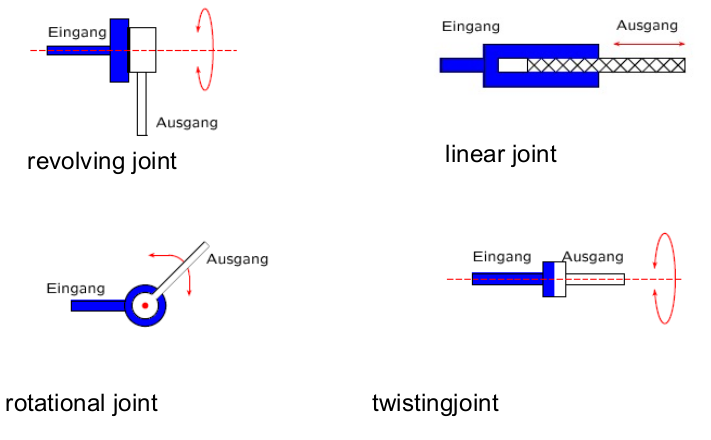
\includegraphics[width=9cm]{sections/imgs/1.png}
\end{center}

Different types of joints connect the links of a manipulator.

\begin{center}
	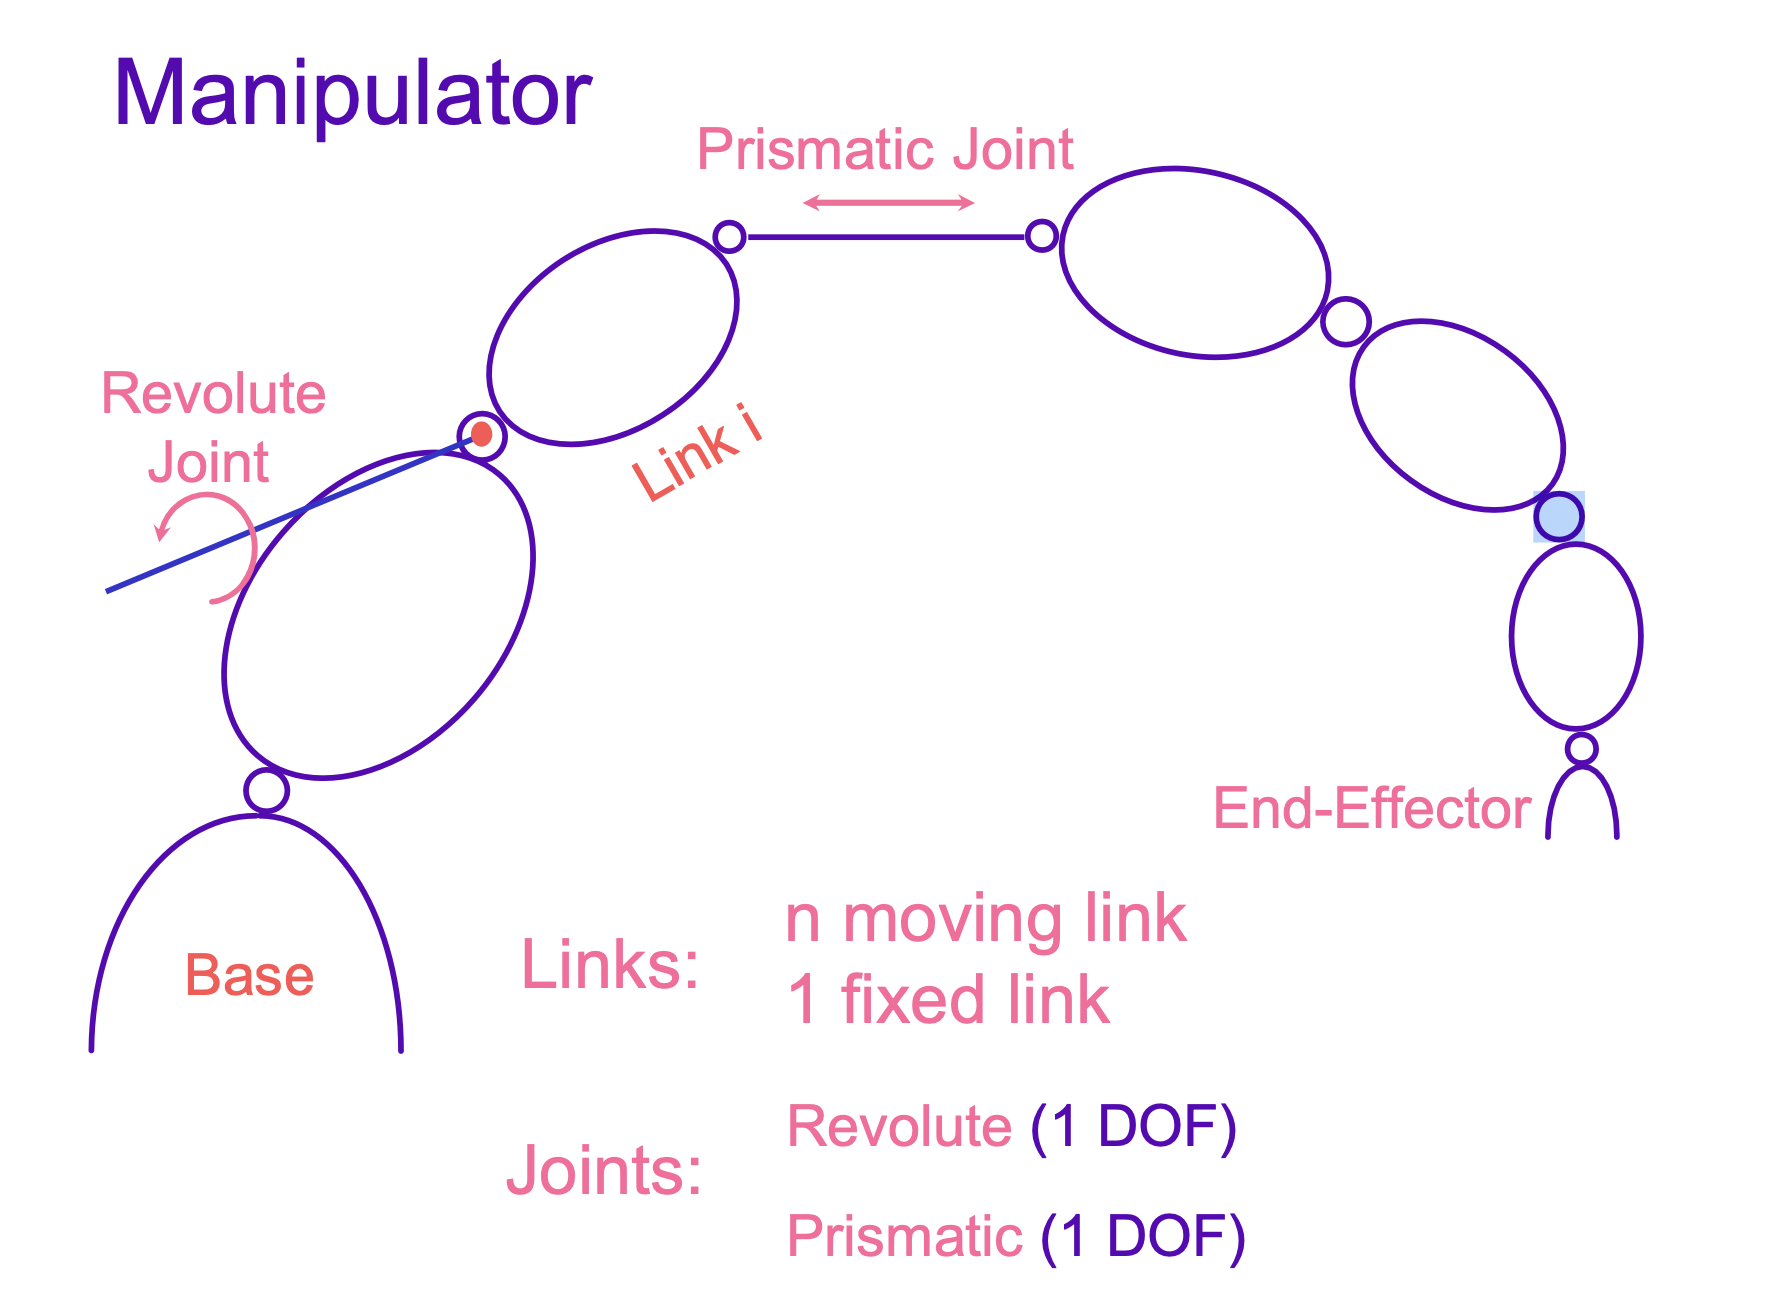
\includegraphics[width=9cm]{sections/imgs/1_manipulator.png}
\end{center}

\section{Forward kinematics}
\subsection{Workspace}
\textbf{Kinematics} is the science of motion that treats motion without regard to the forces which cause it. One studies position, velocity, acceleration, and all higher order derivatives of position variables.

The existence or nonexistence of a kinematic solution defines the \textbf{workspace} of a given manipulator. If a solution doesn't exist, this means that the desired position/orientation lies outside of the manipulator's workspace. In other words, the workspace consists of all points that are reachable by the end-effector.

\subsubsection{Configuration}

The \textbf{configuration} of a moving object is a specification of the position of \textbf{every} point on the object. 

The \textbf{dimension of a config space} is the minimum number of parameters needed to specify the configuration of the object completely (also called the number of degrees of freedom of a moving object).

\subsubsection{Degrees of freedom}
The number of \textbf{degrees of freedom} that a manipulator possesses is the number of independent position variables that would have to be specified in order to locate all parts of the mechanism. E.g., industrial robotic manipulators often have as many d.o.f. as their number of joints, since each joint has one d.o.f. (and has 5 constraints).

\subsubsection{Right-hand-rule}
The signs of angles are determined by the direction of the fingers, when the thumb is pointing in the axis direction. Fingers also show the order of axis.

\begin{center}
	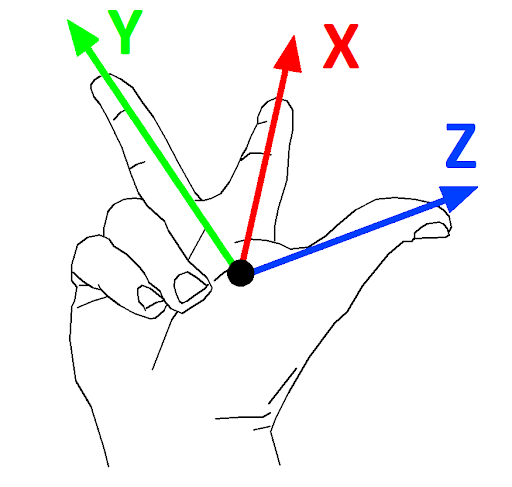
\includegraphics[width=5cm]{sections/imgs/2_right_hand_rule.png}
\end{center}

\subsection{Spatial descriptions}

We attach a coordinate system to a body and give a description of this coordinate system relative to the reference system. In Figure 2.2, system $B$ has been attached to the body, and its description relative to $A$ is given through its positions and orientation relative to $A$. 

\begin{center}
	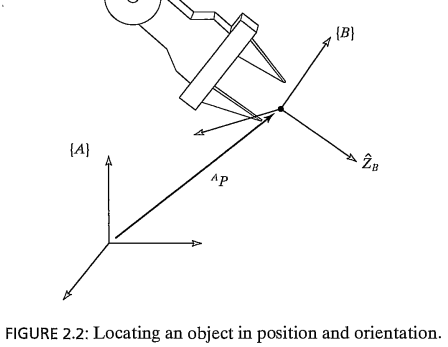
\includegraphics[width=9cm]{sections/imgs/2.png}
\end{center}

\subsubsection{Position}
\textbf{Description of a position:} Since many coordinate systems will be used, one has to define to which system a vector refers, e.g.,

\[^{A}\vect{p} = 
	\begin{bmatrix} p_x\\p_y\\p_z \end{bmatrix}, \] where $^{A}\vect{p}$ is a vector referring to coordinate system $A$.

\subsubsection{Orientation}
\textbf{Description of an orientation:} 
We stack three unit vectors (they specify the principal directions of the coord system) as columns, yielding the \textbf{rotation matrix:} 

\begin{center}
	$^{A}_{B}R = [^{A}\hat{X}_{B}\ ^{A}\hat{Y}_{B}\ ^{A}\hat{Z}_{B}] = 
	\begin{bmatrix} r_{11} & r_{12} & r_{13} \\ r_{21} & r_{22} & r_{23} \\ r_{31} & r_{32} & r_{33} \end{bmatrix} =\ ^{B}_{A} R^{-1} =\ ^{B}_{A} R^T$ \\
\end{center}
The rotation matrix has three constraints:
\begin{itemize}
	\item $|^{A}\hat{X}_{B}| = |^{A}\hat{Y}_{B}| = |^{A}\hat{Z}_{B}| = 1$
	\item $^{A}\hat{X}_{B} \cdot\ ^{A}\hat{Y}_{B} =\ ^{A}\hat{X}_{B} \cdot\ ^{A}\hat{Z}_{B} =\ ^{A}\hat{X}_{B} \cdot\ ^{A}\hat{Z}_{B} = 0$
	\item $\det{R} = 1$
\end{itemize}	
	
It describes the orientation of frame $B$ relative to frame $A$, i.e. it is used as a \textit{mapping} to \textbf{change the description of a vector from frame to frame}. Since we have unit magnitude and the vectors are orthogonal, the transposed matrix describes the orientation of system A written in B. These are orthonormal and length-preserving linear transformations. Also, rotation matrices preserve angles between vectors, i.e. $cos(\angle (\vect{p}, \vect{q})) = cos(\angle (R\vect{p}, R\vect{q}))$. The projection of a vector $\hat{X}_B$ in coord system $B$ into coord system $A$ is derived from the dot product with the principal directions of the coord frame of $A$, hence the graphic.
	
\begin{center}
	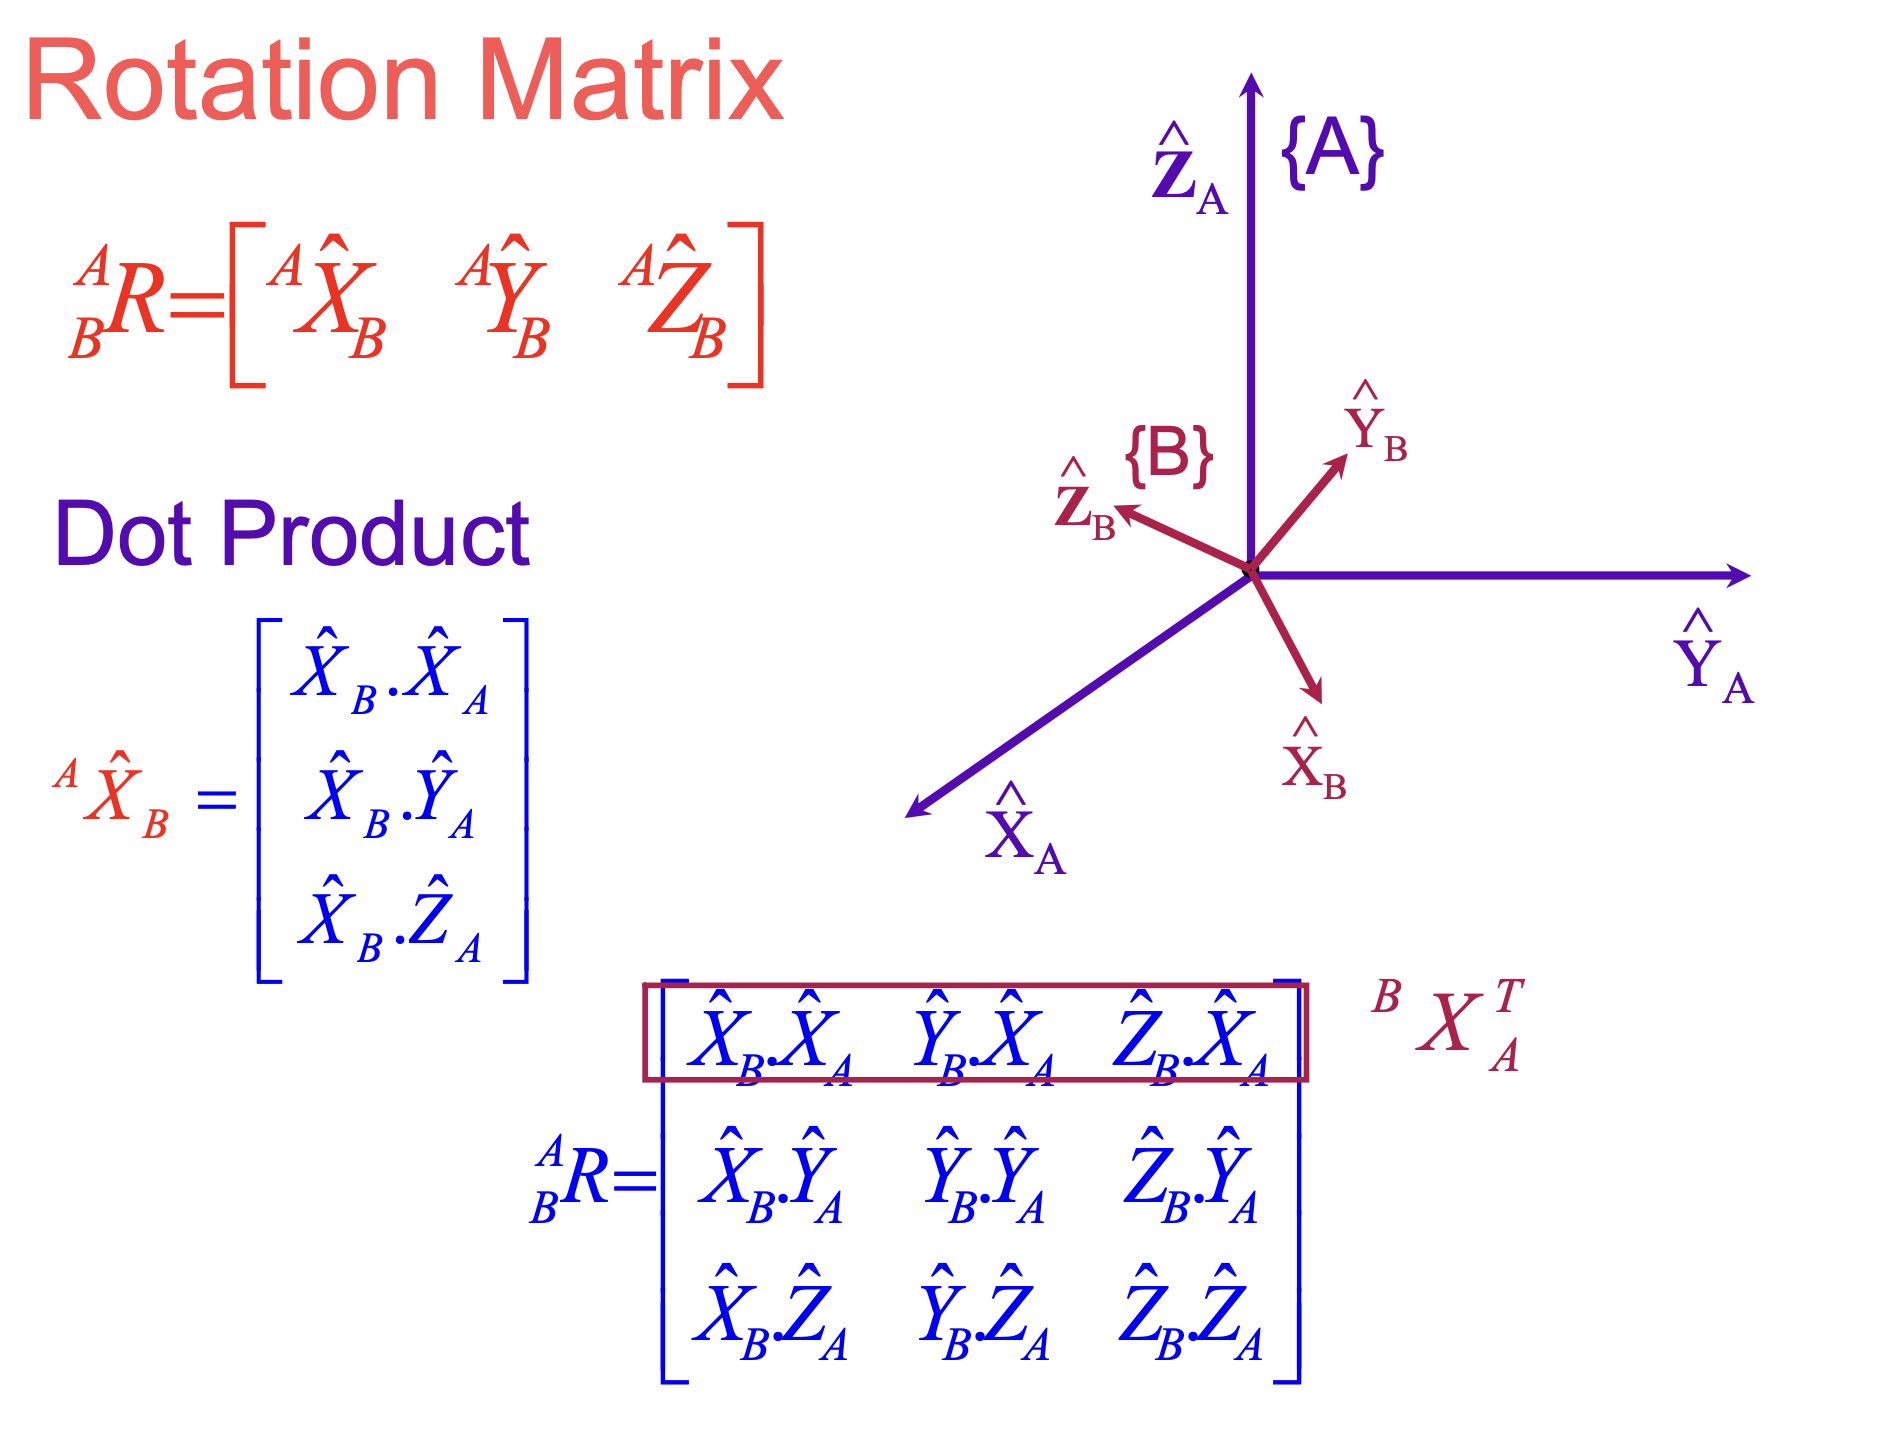
\includegraphics[width=9cm]{sections/imgs/2_rotation_matrix.png}
\end{center}

Besides mappings, another use case of rotation matrices is in the form of (rotational)\textit{operators} to move points within the same frame.

\subsubsection{Euler angles}
There is an issue when expressing orientations with a rotation matrix: When attempting to follow a trajectory in space by interpolating a current orientation from a start until a final orientation, the intermediary orientations are going to violate the constraints of the rotation matrix. Another possible description of a frame $B$ uses a \textit{three-angle-representation}. It works as follows: Frame $B$ coincides with a known frame $A$. Rotate $B$ first
\begin{itemize}
	\item about $ \hat{X}_{A} $ by an angle \(\gamma\), then about
	\item $ \hat{Y}_{A} $ by an angle \(\beta\), and finally about
	\item $ \hat{Z}_{A} $ by \(\alpha\).
\end{itemize}
If, each of the three rotations takes place about an axis in the fixed reference frame $A$, we call these angles \textit{X-Y-Z fixed angles}. An alternative representation uses angles that are relative to the previously changed coordinate frame, so-called \textbf{Euler angles}.

\begin{center}
	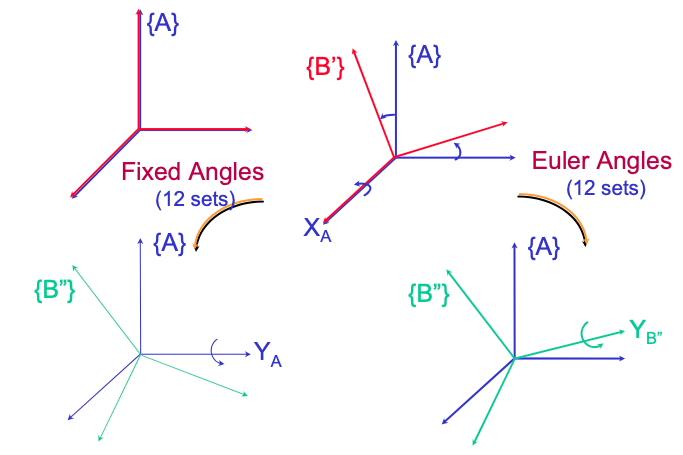
\includegraphics[width=10cm]{sections/imgs/2_fixed_relative_angles.png}
\end{center}

The next figure shows three subsequent rotations of a frame around the fixed axes $\hat X_A$, $\hat Y_A$ and $\hat Z_A$.

\begin{center}
	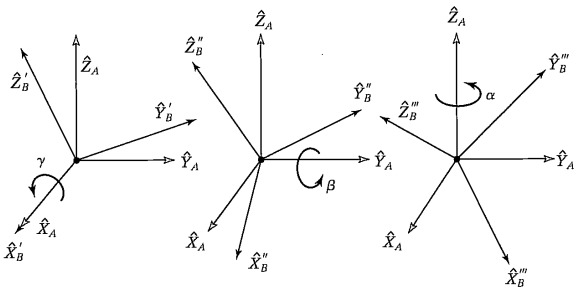
\includegraphics[width=10cm]{sections/imgs/9.png}
\end{center}

The combined rotation matrix is $^{A}_{B}R =\ ^{A}_{B'}R \cdot \ ^{B'}_{B''}R \cdot \ ^{B''}_{B}R$, which is cumbersome to compute. Instead, we define:

\begin{align*}
{ }_{B}^{A} R_{X Y Z}(\gamma, \beta, \alpha) &=R_{Z}(\alpha) R_{Y}(\beta) R_{X}(\gamma) \\
&=\left[\begin{array}{ccc}
\cos \alpha & -\sin \alpha & 0 \\ \sin \alpha & c \alpha & 0 \\ 0 & 0 & 1
\end{array}\right]\left[\begin{array}{ccc}
\cos \beta & 0 & \sin \beta \\ 0 & 1 & 0 \\ -\sin \beta & 0 & \cos \beta
\end{array}\right]\left[\begin{array}{ccc} 1 & 0 & 0 \\ 0 & \cos \gamma & -\sin \gamma \\
0 & \sin \gamma & \cos \gamma
\end{array}\right] \\
&= \left[\begin{array}{ccc}
\cos \alpha \cos \beta & \cos \alpha \sin \beta \sin \gamma-\sin \alpha \cos \gamma & \cos \alpha \sin \beta \cos \gamma+\sin \alpha \sin \gamma \\
\sin \alpha \cos \beta & \sin \alpha \sin \beta \sin \gamma+\cos \alpha \cos \gamma & \sin \alpha \sin \beta \cos \gamma-\cos \alpha \sin \gamma \\
-\sin \beta & \cos \beta \sin \gamma & \cos \beta \cos \gamma
\end{array}\right]
\end{align*}

When rotating a frame with Euler angles in the order of $Z$-$Y$-$X$, they produce the same combined rotation as $X$-$Y$-$Z$ fixed angles, i.e. $R_{Z^{\prime} Y^{\prime} X^{\prime}}(\alpha, \beta, \gamma)=R_{X Y Z}(\gamma, \beta, \alpha)$ for the same values of $(\alpha, \beta, \gamma)$. This next graphic shows the rotation using Euler angles:

\begin{center}
	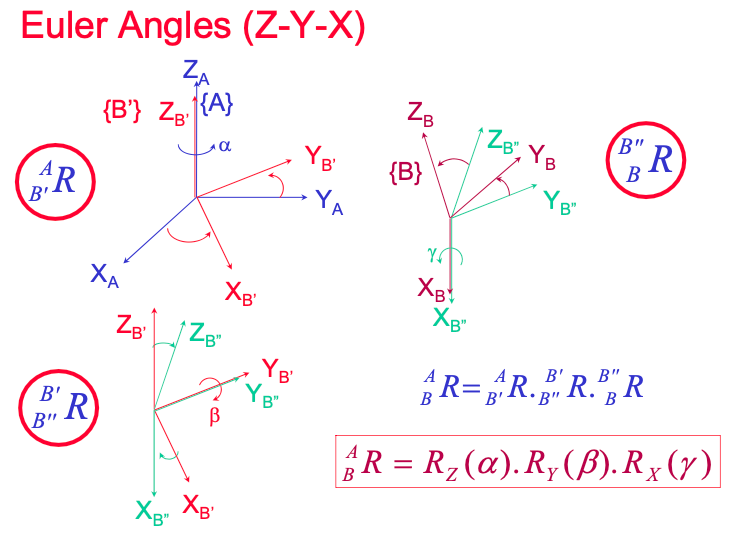
\includegraphics[width=10cm]{sections/imgs/2_euler_angles.png}
\end{center}

\textbf{Inverse problem:} Given $^{A}_{B}R$ find the $X$-$Y$-$Z$ fixed angles $(\alpha, \beta, \gamma)$. Let
\[{ }_{B}^A R_{X Y Z}(\gamma, \beta, \alpha)=\left[\begin{array}{lll}
r_{11} & r_{12} & r_{13} \\
r_{21} & r_{22} & r_{23} \\
r_{31} & r_{32} & r_{33}
\end{array}\right] \]

\begin{minipage}{0.4\textwidth}
Then:

\begin{align*}
&\beta=\operatorname{Atan} 2\left(-r_{31}, \sqrt{\left.r_{11}^{2}+r_{21}^{2}\right.}\right) \\
&\alpha=\operatorname{Atan} 2\left(r_{21} / \cos \beta, r_{11} / \cos \beta\right) \\
&\gamma=\operatorname{Atan} 2\left(r_{32} / \cos \beta, r_{33} / \cos \beta\right)
\end{align*}
	
\end{minipage}
\begin{minipage}{0.49\textwidth}
	\[ \operatorname{Atan} 2(a, b)= \begin{cases}\arctan \left(\frac{a}{b}\right) & \text { if } b>0 \\ \frac{\pi}{2} & \text { if } b=0, a>0 \\ \text { undefined } & \text { if } b=0, a=0 \\ -\frac{\pi}{2} & \text { if } b=0, a<0 \\ \arctan \left(\frac{a}{b}\right)+\pi & \text { if } b<0\end{cases} \]
\end{minipage}
\vspace{0.5cm}

 Note that for every parameter $(\alpha, \beta, \gamma)$ there are values which cause a singularity in this computation (e.g. for $\cos \beta = 0$).

\subsubsection{Unit quaternions (Euler parameters)}
Another representation of orientation is by means of four values called the \textbf{Euler parameters}. It can be shown that every rotation can be expressed as one rotation of $\theta$ around a single axis $K = [k_x\ k_y\ k_z]^T$. This is also known as the \textit{equivalent angle-axis representation}. 

\begin{center}
	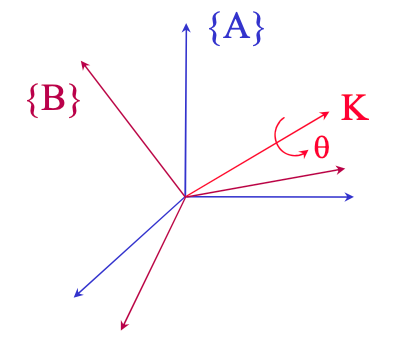
\includegraphics[width=4cm]{sections/imgs/2_equivalent_angle_axis.png}
\end{center}

The Euler parameters are given by

\[ (\varepsilon_1 , \varepsilon_2 , \varepsilon_3 , \varepsilon_4) = ( k_{x} \sin \frac{\theta}{2}, k_{y} \sin \frac{\theta}{2}, k_{z} \sin \frac{\theta}{2}, \cos \frac{\theta}{2})  \]

and 
\[ \epsilon_{1}^{2}+\epsilon_{2}^{2}+\epsilon_{3}^{2}+\epsilon_{4}^{2}=1 \]

This $4 \times 1$ vector is known as a unit quaternion, the orientation it describes could be visualized as a point on a unit hypersphere in four-dimensional space. It turns out that the orientation representation through Euler parameters does not have a singularity.


\subsection{Spatial transformations}
\textit{Problem:} We know the definition of a vector with respect to some frame $B$ and we would like to express it with respect to another frame $A$, where the origins of the two frames are coincident. We can compute this, if we know a description of the orientation of $B$ relative to $A$. Then, \[^{A} P = {^{A}_{B}}R\ {^{B}}P \] computes what a \textbf{vector that is expressed in coordinate system B ``looks like'' if observed from system A}.

\begin{center}
	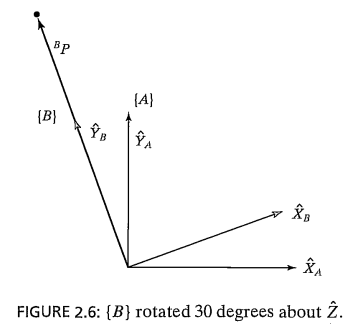
\includegraphics[width=5cm]{sections/imgs/4.png} 
	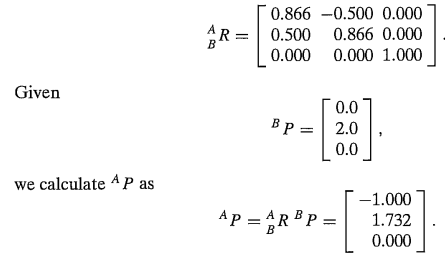
\includegraphics[width=7cm]{sections/imgs/5.png}	
\end{center}

Now, the \textbf{general case}, where the systems don't have the same origin, but B is shifted by $P_{BORG}$ from the origin (or $^{A}P_{BORG}$ when expressed in $A$):

$$^{A}P =\ ^{A}_{B}R\ ^{B}P + \ ^{A}P_{BORG}\ $$ 

\begin{center}
	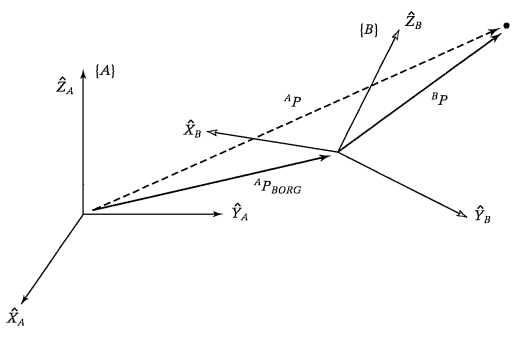
\includegraphics[width=6cm]{sections/imgs/6.png}
\end{center}

Computing a position of a point connected by multiple subsequent links of a manipulator with individual coordinate frames, involves the multiplication of sums given by the general transform equation. This is because \textit{rotation} and \textit{translation} are both needed to propagate from one frame to another. To simplify this calculation, a \textbf{homogeneous transform} combines rotation and translation into a matrix $_{B}^{A}T$, such that: ${}^{A}P={}_{B}^{A}T\ ^{B}P$. Therefore, the homogeneous transform is a \textit{general operator}.

\begin{center}
	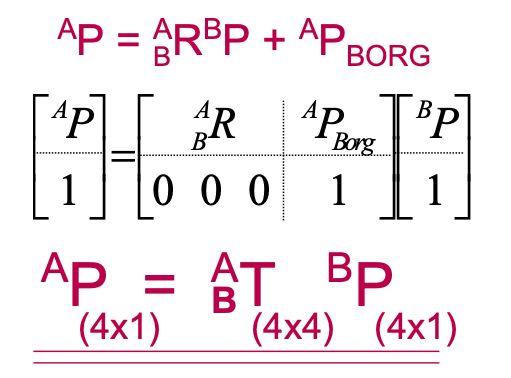
\includegraphics[width=4cm]{sections/imgs/2_homogeneous_transform.png}
\end{center}

Due to the generality of the homogeneous transform, it can be interpreted in different ways: 1.) as a description of a frame $\{B\}=\{_{B}^{A}R \ \ ^{A}P_{BORG}\}$; 2.) as a mapping of a point in frame $B$ to frame $A$; 3.) as an operator to rotate and translate a point in the same frame. This is an example for the second case:

\begin{center}
	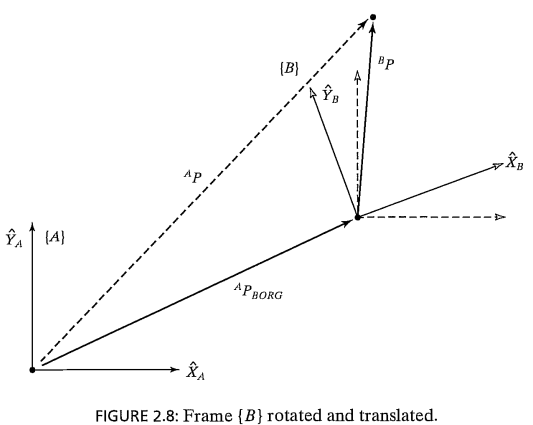
\includegraphics[width=6cm]{sections/imgs/7.png}
	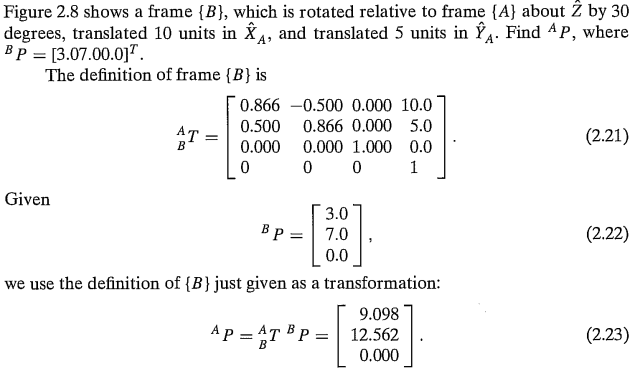
\includegraphics[width=8cm]{sections/imgs/8.png}
\end{center}
 
Inverse of the homogeneous transform:

\begin{center}
	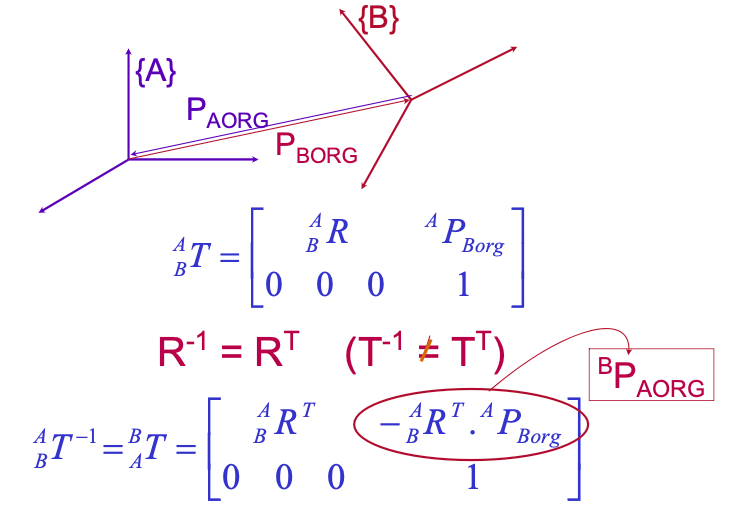
\includegraphics[width=7cm]{sections/imgs/2_inverse_transform.png}
\end{center}

Compound transformation:

\begin{center}
	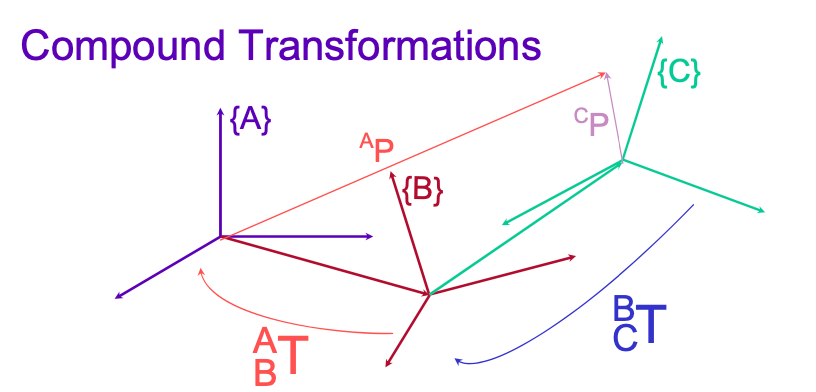
\includegraphics[width=7cm]{sections/imgs/2_compound_transformation_1.png}
	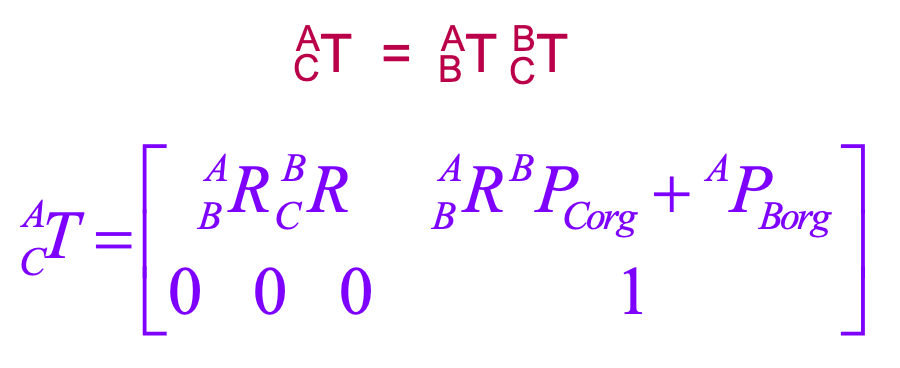
\includegraphics[width=6cm]{sections/imgs/2_compound_transformation_2.png}
\end{center}

Transform equation: ${}_{B}^{A}T \ {}_{C}^{B}T \ {}_{D}^{C}T \ {}_{A}^{D}T= I$.

\subsection{Forward kinematics}
Forward kinematics solves the static geometrical problem of computing the position and the orientation of the end-effector of the manipulator. Specifically, given a \textbf{set of joint angles}, the forward kinematic problem is to compute the position and orientation of the tool frame relative to the base frame.

\subsubsection{Denavit-Hartenberg Convention}
The homogeneous transform between consecutive frames of links is represented via only 4 D-H-parameters (x-rot, x-trans, z-trans, z-rot). In general, 6 parameters are needed to represent an arbitrary rigid body transformation! Thus, a restriction of it is, that it \textbf{cannot represent a rotation around the $y$-axis and that the $y$- and $z$-position are coupled}.

Procedure for deriving the D-H-parameters:

\begin{center}
	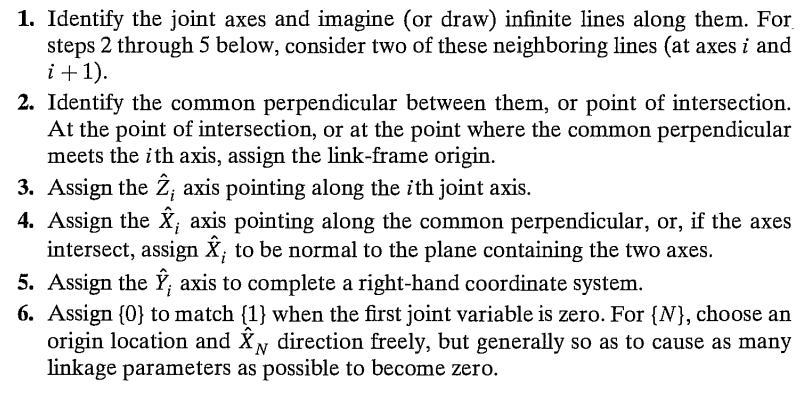
\includegraphics[width=13cm]{sections/imgs/10.png}\\
	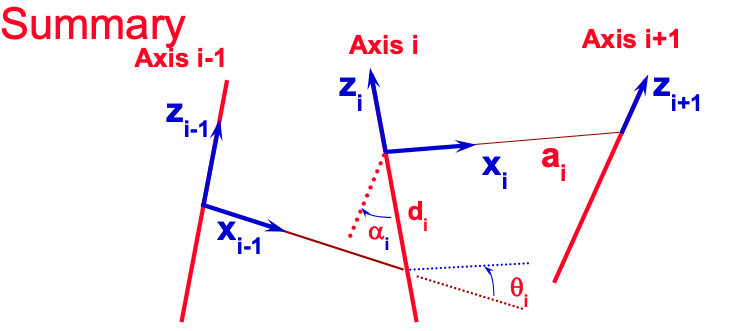
\includegraphics[width=7cm]{sections/imgs/2_dh_params.png}
	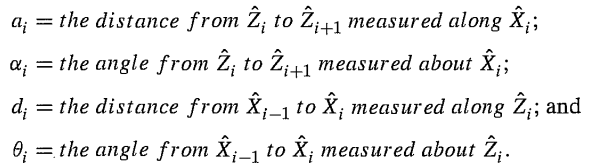
\includegraphics[width=9cm]{sections/imgs/11.png}
\end{center}

Among the four D-H-parameters are three fixed link parameters and one joint variable, which is $\theta_i$ for a revolute joint or $d_i$ for a prismatic joint. The D-H-parameters are plugged into homogenous transformation matrices, which represent the single transformations between the frames of subsequent links. Then, we can propagate through all homogeneous transformations to calculate the position and orientation of the end-effector. Hereafter, the above described procedure is detailed further:\\

\begin{figure*}[h]
	\centering
	\subfloat[Identify the joint axes; consider axes $i$ and $i-1$. By convention, a joint axis points \textbf{in the direction of the rotation/ movement} for revolute/ prismatic joints.]{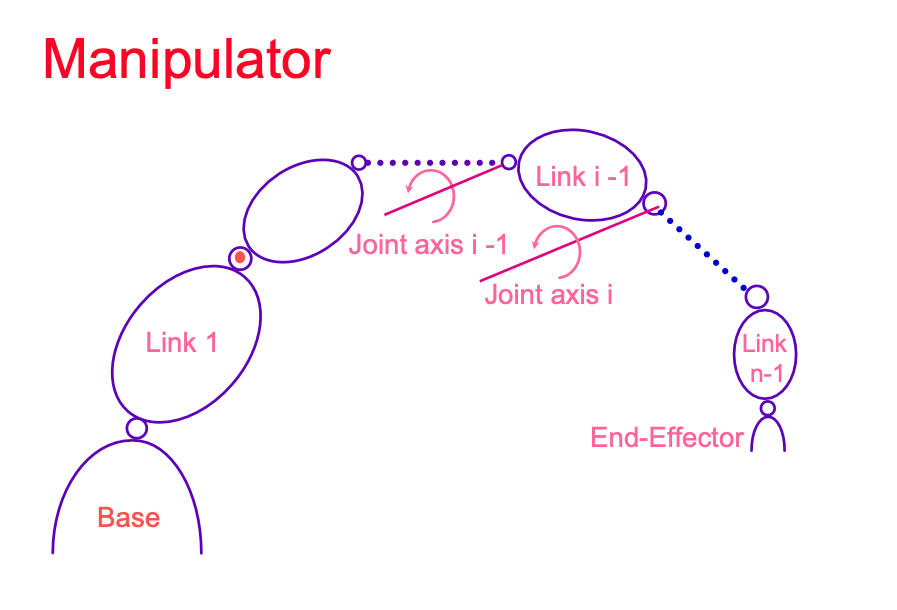
\includegraphics[width=.45\textwidth]{sections/imgs/2_dh_1.png}}
	\hfill
	\subfloat[Identify the common perpendicular. If the axes intersect, the common perpendicular is a normal through the plane they span and the direction of $\alpha_i$ is determined by the direction of this normal. \textbf{$a_i$ and $\alpha_i$ describe the $i$th link}. (``We rotate axis $i-1$ around the normal about $\alpha$ so that it coincides with axis $i$. This aligns the $Z$-axes.'')]{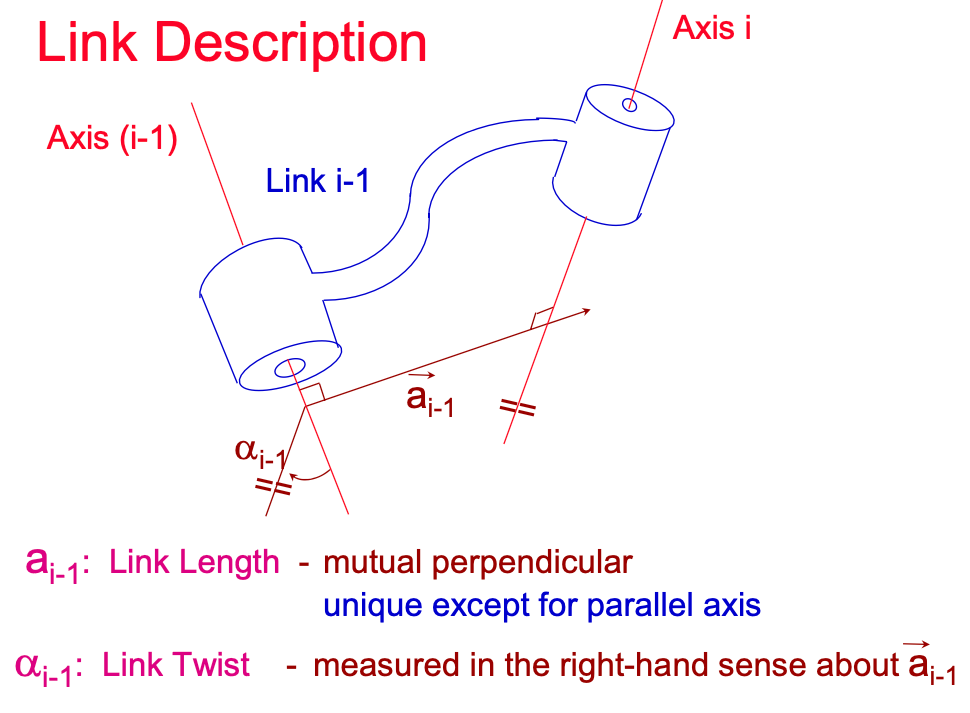
\includegraphics[width=.45\textwidth]{sections/imgs/2_dh_2.png}}\\
\end{figure*}

\begin{figure*}[h]
	\ContinuedFloat
	\centering
	\subfloat[\textbf{$d_i$ and $\theta_i$ describe the $i-1$th link connection}. If the axes of link $i-1$ and link $i$ are parallel, the origin of a coordinate frame $\{i-1\} $ should be attached, such that $d_i=0$. (``$\theta_i$ aligns the $X$-axes by rotation around $Z_i$.'')]{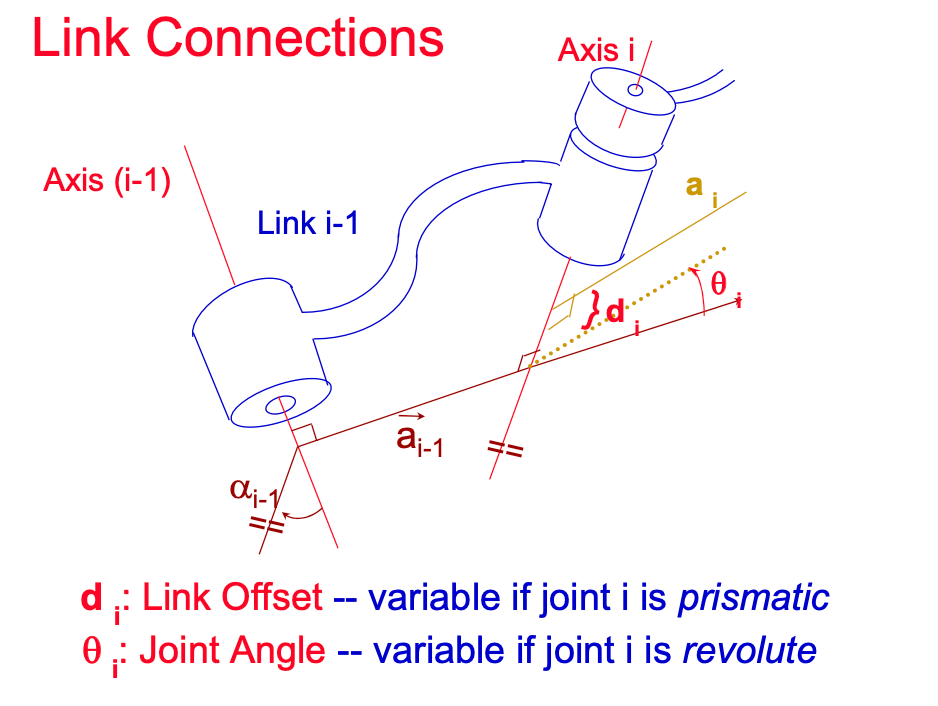
\includegraphics[width=.45\textwidth]{sections/imgs/2_dh_3.png}}
	\hfill
	\subfloat[Attach $i$th frame, such that $\hat Z_i$ is in the direction of the $i$th joint axis and $\hat X_i$ points along the common perpendicular (if $\hat Z_{i-1}$ and $\hat Z_i$ intersect, choose $\hat X_{i-1}$, such that $\alpha_{i-1}>0$). $\hat Y_i$ completes the right-hand frame.]{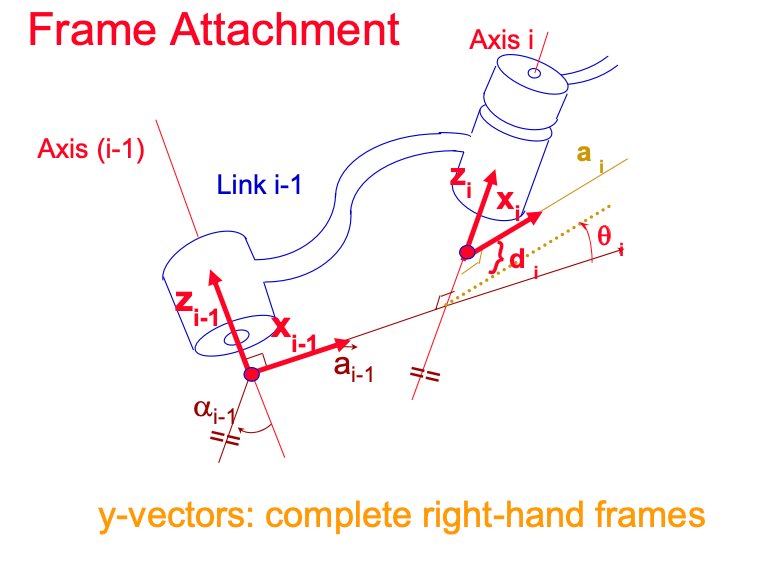
\includegraphics[width=.45\textwidth]{sections/imgs/2_dh_4.png}}\\
\end{figure*}

\begin{figure}[h]
	\ContinuedFloat 
	\centering
	\subfloat[$a_i$ and $\alpha_i$ depend on joint axes $i$ and $i+1$. Thus, select axes $0$ and $n+1$, such that $a_0=a_n=0$ and $\alpha_0=\alpha_n=0$ (by making axis $0$ coincident with axis $1$ and axis $n+1$ coincident with axis $n$). This simplifies the forward kinematics.]{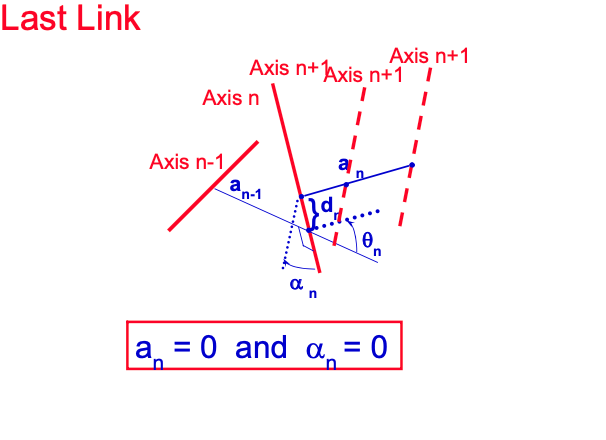
\includegraphics[width=.45\textwidth]{sections/imgs/2_dh_5.png}}
	\hfill
	\subfloat[$\theta_i$ and $d_i$ depend on joint axes $i$ and $i-1$. Again, select axes $0$ and $n+1$, such that depending on the joint type $a_0$ or $\theta_0=0$ and $a_n$ or $\theta_n=0$ (by coinciding axes and moving the intersection point that becomes the origin of the frame so that $d=0$ or orienting the axis so that $\theta=0$). ]{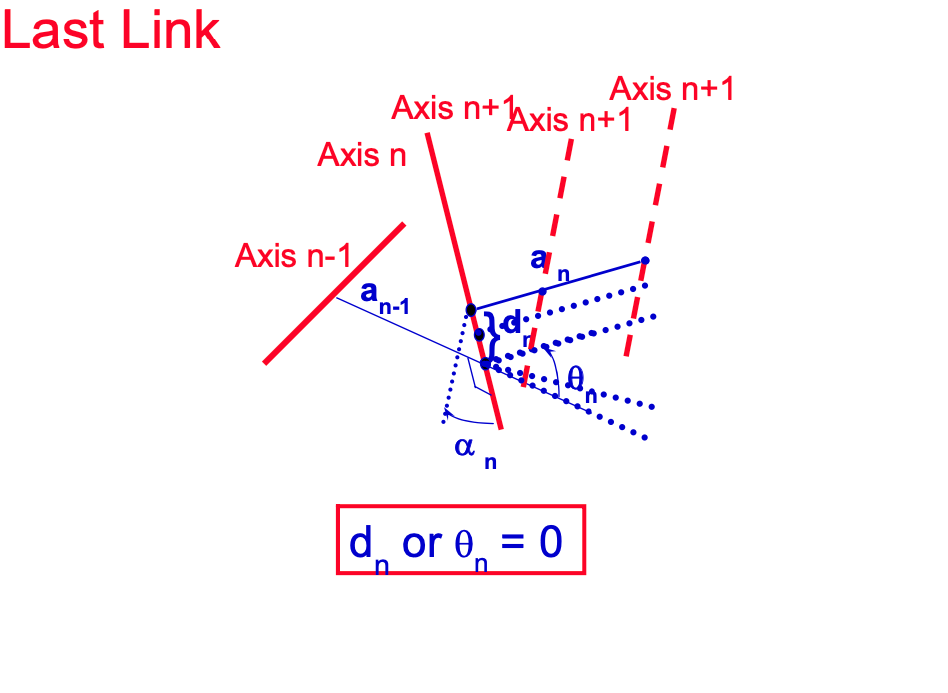
\includegraphics[width=.45\textwidth]{sections/imgs/2_dh_6.png}}
\end{figure}
 
\begin{figure}[h]
	\ContinuedFloat 
	\centering
	\subfloat[$\{0\}$ is assigned, such that is equals $\{1\}$ when the first joint variable is $0$.]{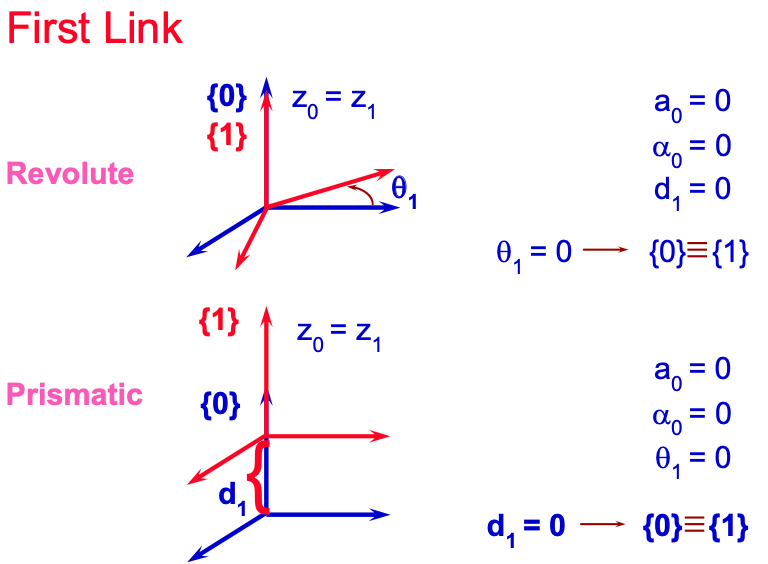
\includegraphics[width=.45\textwidth]{sections/imgs/2_dh_7.png}}
	\hfill
	\subfloat[Assign $\{N\}$, such that the most parameters are $0$.]{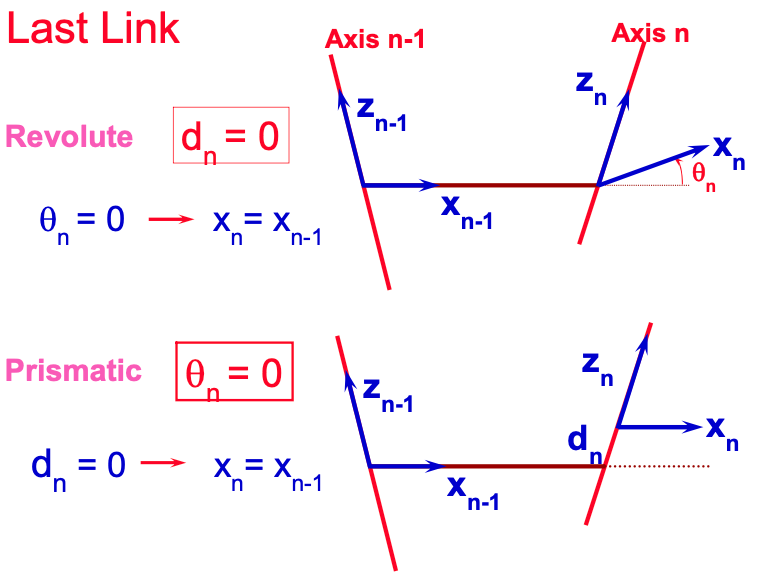
\includegraphics[width=.45\textwidth]{sections/imgs/2_dh_8.png}}
\end{figure}

\FloatBarrier

Then, the forward kinematics of a single link using the D-H-parameters derive as follows:

\begin{figure}[h]
	\centering
	\subfloat[To obtain $^{i-1}_{i}T$: Translate along $Z_{i}$ about $d_i$ ($\rightarrow \{P\} $), then rotate around $Z_i$ about $\theta_i$ ($\rightarrow \{Q\} $), then translate along $X_{i-1}$ about $a_{i-1}$ ($\rightarrow \{R\} $) and finally rotate around $X_i$ about $\alpha_i$ ($\rightarrow \{i-1\} $). This results in the homogeneous transform for a single link from $\{i\} $ to $\{i-1\} $ and also works in the other direction to compute the inverse homogeneous transform.]{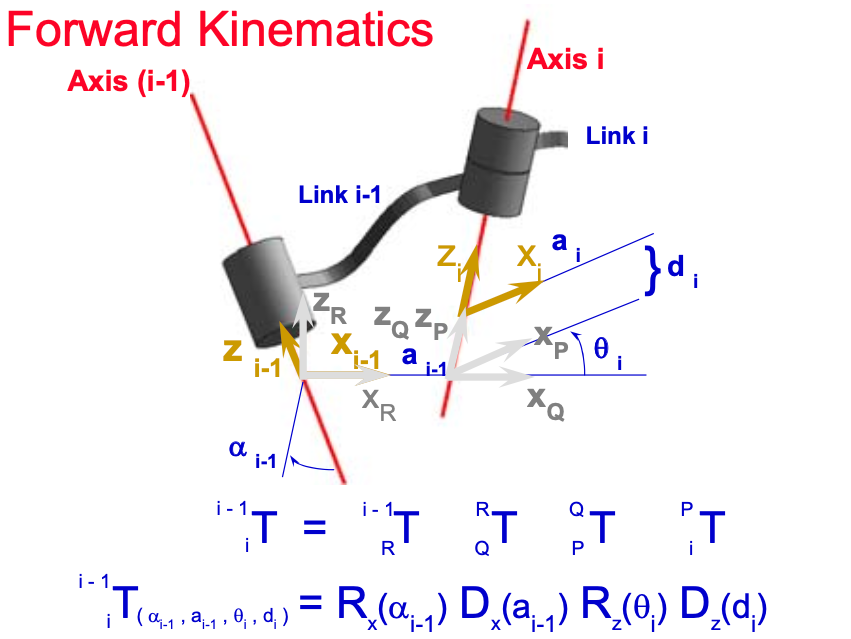
\includegraphics[width=.45\textwidth]{sections/imgs/2_dh_fkin_1.png}}
	\hfill
	\subfloat[The \textbf{homogeneous transformation from link $i$ to link $i-1$} (the formula in the slide should say $i$ instead of $1$).]{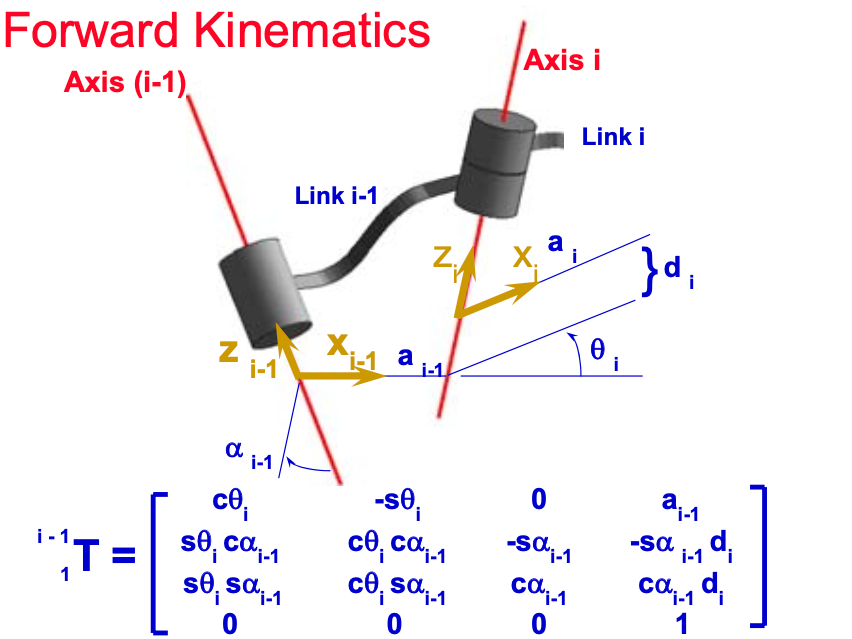
\includegraphics[width=.45\textwidth]{sections/imgs/2_dh_fkin_2.png}}\\
	\subfloat[The homogeneous transformation which transforms points from the frame of link $N$ to the frame of link $0$.]{
\includegraphics[width=.45\textwidth]{sections/imgs/2_dh_fkin_3.png}}
	
\end{figure}

Note, that the homogeneous transform ${}^{i-1}_iT$ cannot express arbitrary rigid body transformations, since no rotation about $\hat{Y}$ is possible.
A good, practical explanation of how to place the coordinate frames at each link, derive the D-H-parameters and compute the homogeneous transformations and forward kinematics is given in \href{https://youtu.be/u79KfNgP1Cc?t=1939}{this video} (based on an example).
\section{Inverse Kinematics}
Recap forward kinematics: Given a joint configuration, find the pose of some part of the robot.\\
Inverse kinematics: Given a pose, figure out the joint configurations.

Input data for the problem is of the form:
\[ T=\left[\begin{array}{cc}
R & t \\
0 \; 0 \; 0 & 1
\end{array}\right] \]
This is a nonlinear problem, thus it's not sure if there is a (unique/multiple/infinite/outside-of-workspace/none) solution. Inverse kinematics are not explicitly discussed the Stanford lecture and there is not particular exercise on it (albeit it is included in the lecture). 

\subsection{Multiplicity of Solutions}
If there are multiple solutions (configurations), choose the closest one:

{\centering 
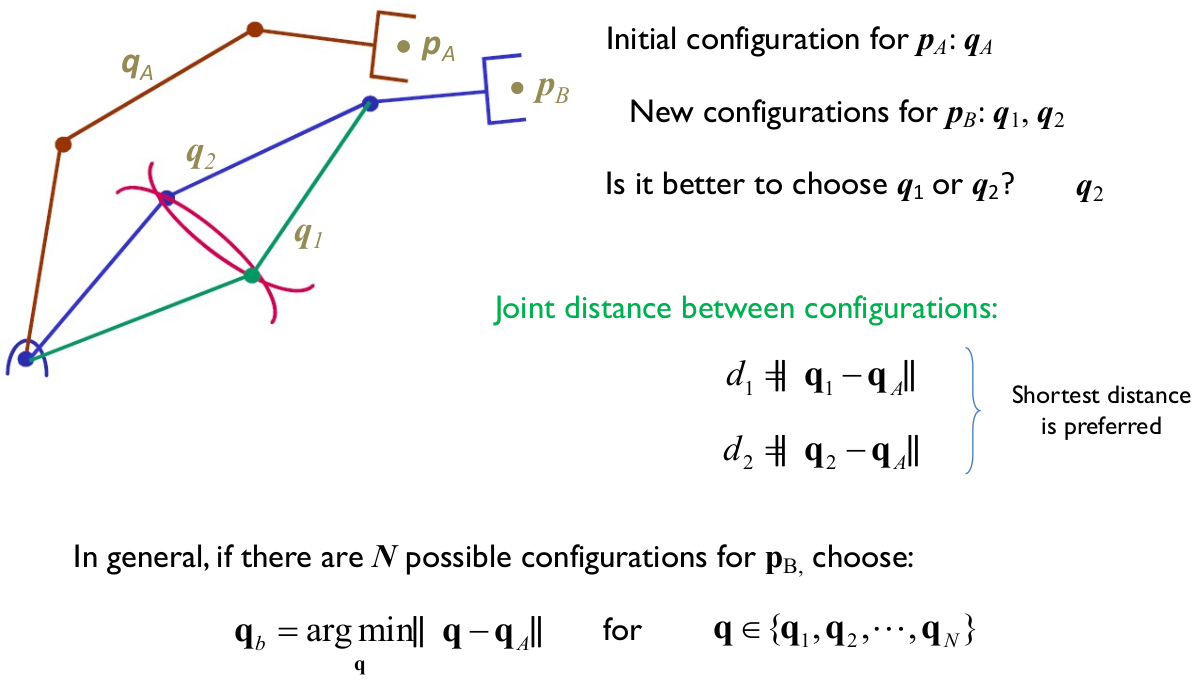
\includegraphics[width=13cm]{sections/imgs/12.png}
\\}
\subsubsection{Redundancy}
{\centering 
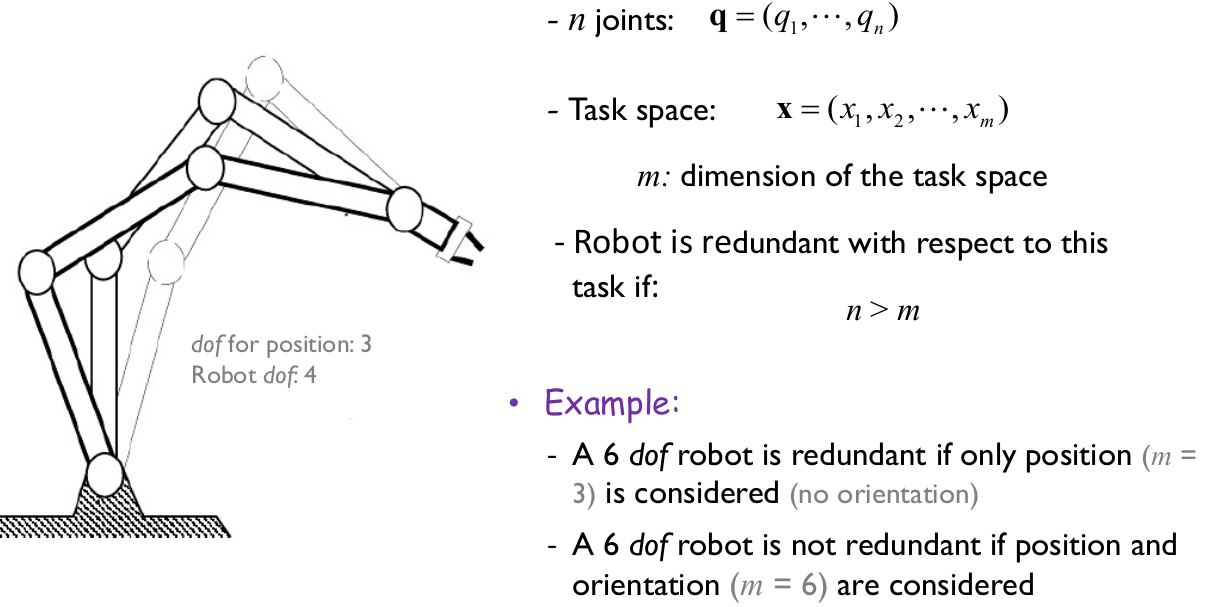
\includegraphics[width=13cm]{sections/imgs/13.png}
\\}

\subsection{Analytic solutions for the inverse kinematics}
\subsubsection{Geometric solution}
\begin{itemize}
	\item only when robot has 3 or less dofs
	\item not a generic solution
\end{itemize}

{\centering 
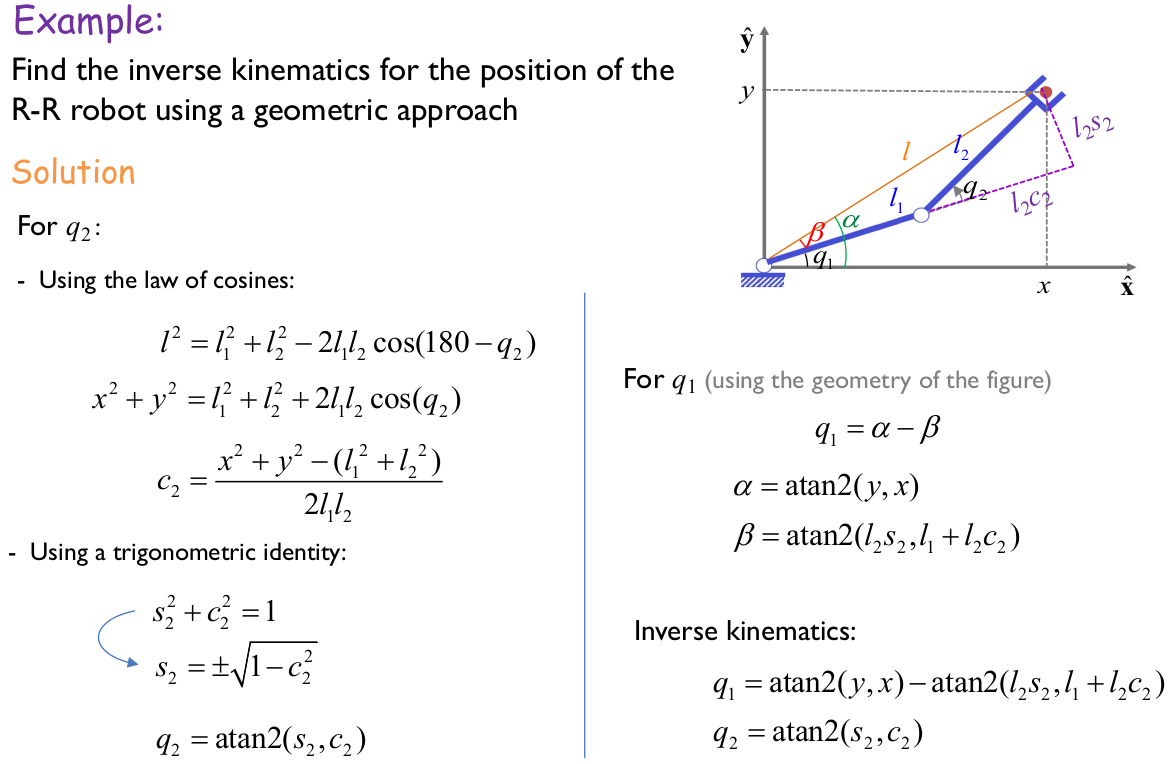
\includegraphics[width=15cm]{sections/imgs/14.png}
\\}

\subsubsection{Algebraic solution}
Solution using algebraic (and polynomial) equations.\\
Given: Formula to find the kinematic equations of an arm easily, given link params. E.g.:

{\centering 
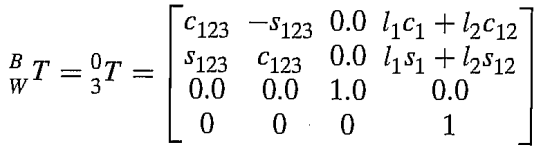
\includegraphics[width=6cm]{sections/imgs/15.png}
\\}

This describes the wrist (manipulator) frame relative to the base frame.\\
We also know what is necessary to describe such a position/orientation:

{\centering 
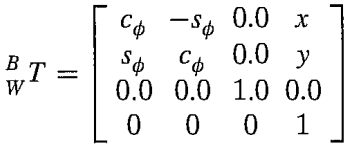
\includegraphics[width=4cm]{sections/imgs/16.png}i
\\}

So just an x-y positon and an angle \(\phi\).
By equating both, we get a set of nonlinear equations, which have to be solved for $ l_1 , l_{2} , \theta $, using magical algebra:

{\centering 
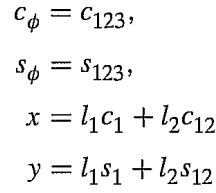
\includegraphics[width=3cm]{sections/imgs/17.png}
\\}

\subsubsection{Example}

\begin{center}
	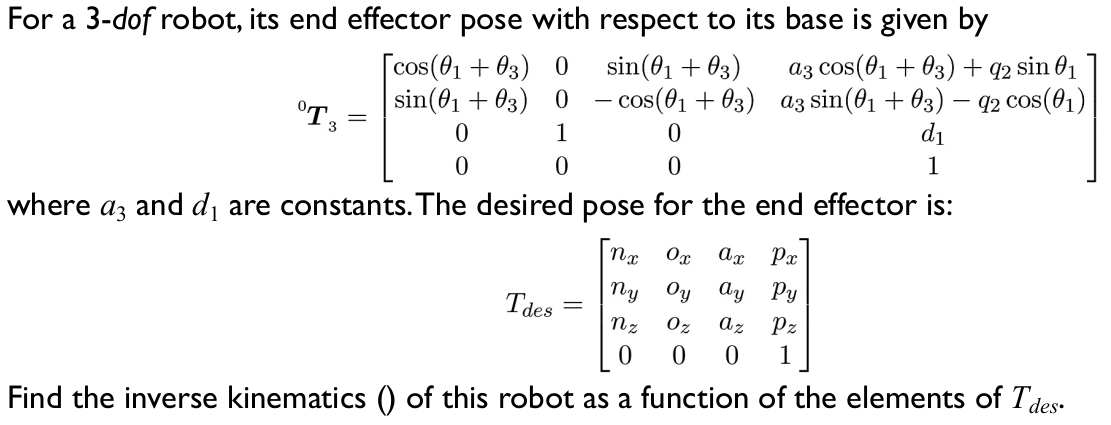
\includegraphics[width=8cm]{sections/imgs/18.png}\\
	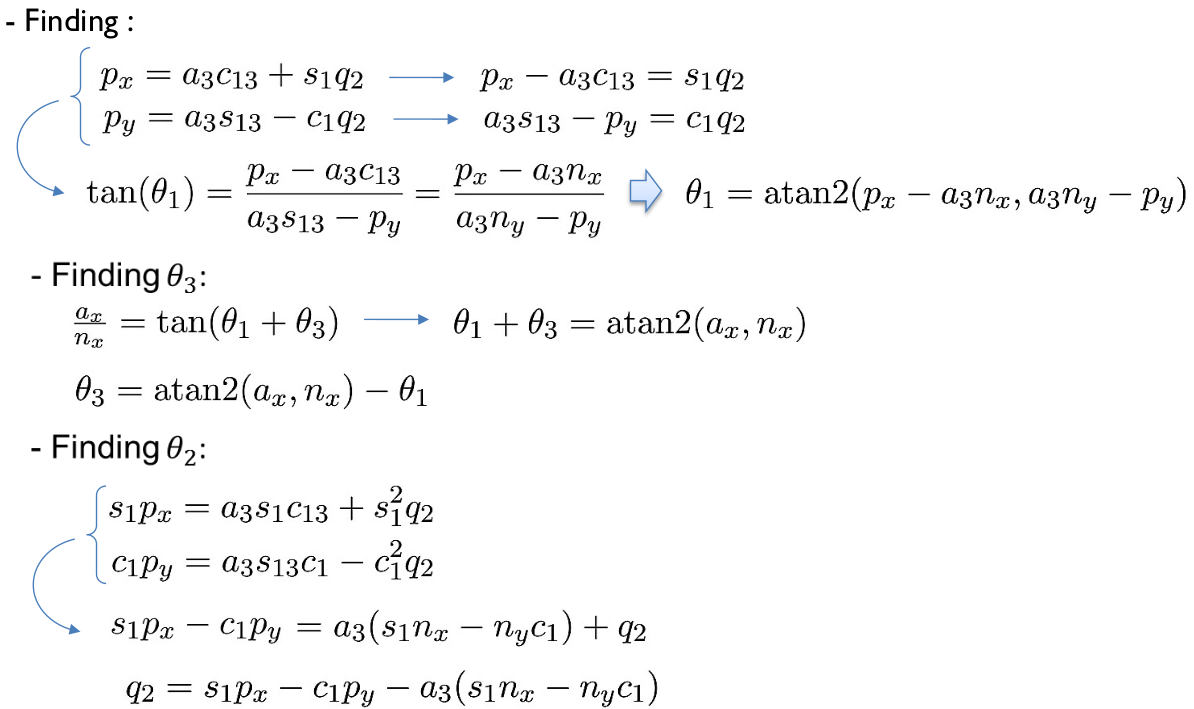
\includegraphics[width=9cm]{sections/imgs/19.png}
\end{center}

\subsection{Numeric solutions to the inverse kinematics}
Mainly used when..
\begin{itemize}
	\item no analytic solution
	\item $ \infty $ solutions
	\item too difficult to find a solution
\end{itemize}
{\centering 
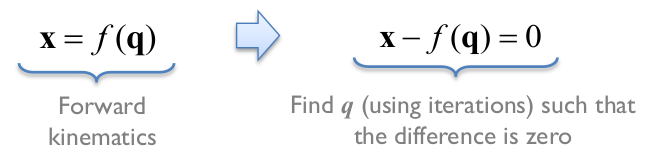
\includegraphics[width=8cm]{sections/imgs/20.png}
\\}
Uses the Jacobian matrix:
\[J (q) = \frac{\partial f (q)}{\partial q} \quad J (q) \in \mathcal{R}^{n \times m}  \]
Where $ n $ is the size of $ q $ (number of joints) and $ m $ is the size of $ x $ (size of task space)

\subsubsection{Newton's Method}

\begin{center}
	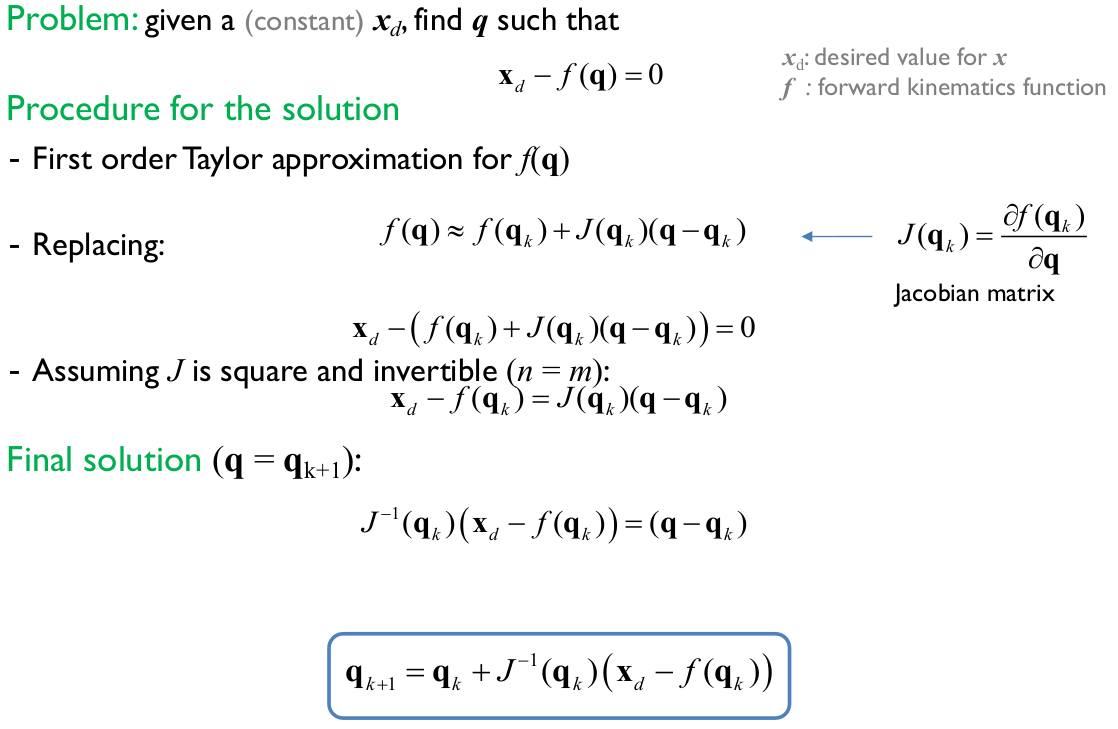
\includegraphics[width=11cm]{sections/imgs/21.png}\\
	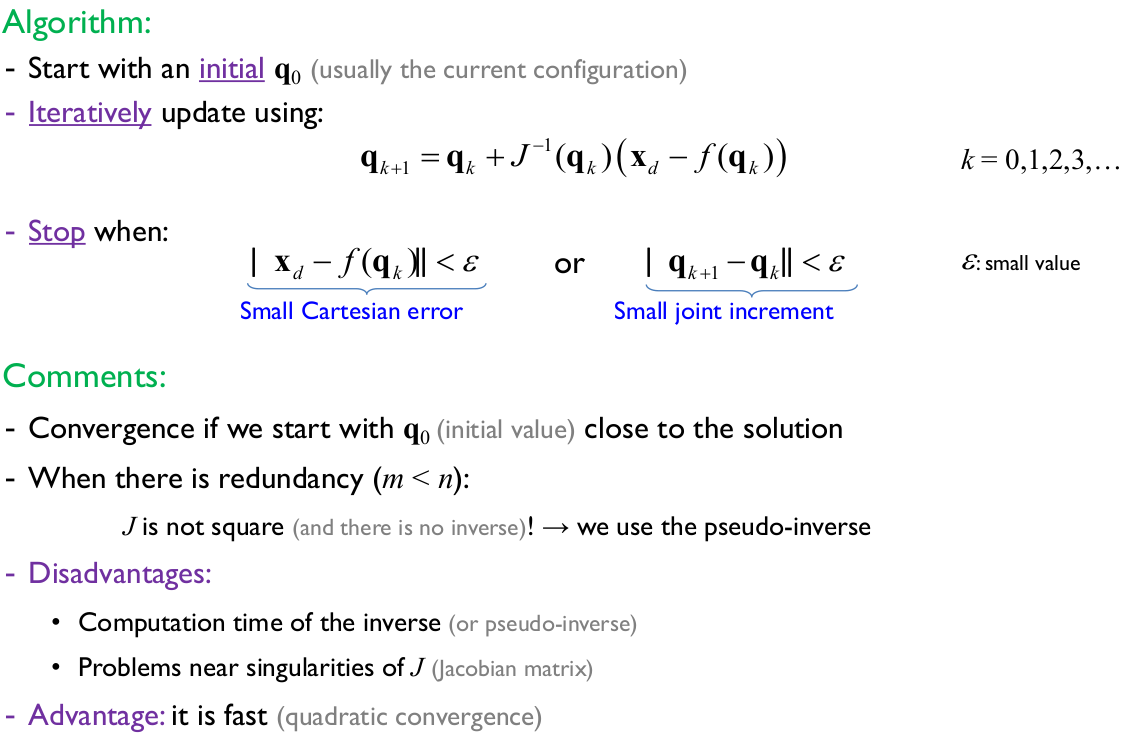
\includegraphics[width=11.4cm]{sections/imgs/22.png}
\end{center}
Example in slides.

\subsubsection{Gradient Descent Method}
\begin{center}
	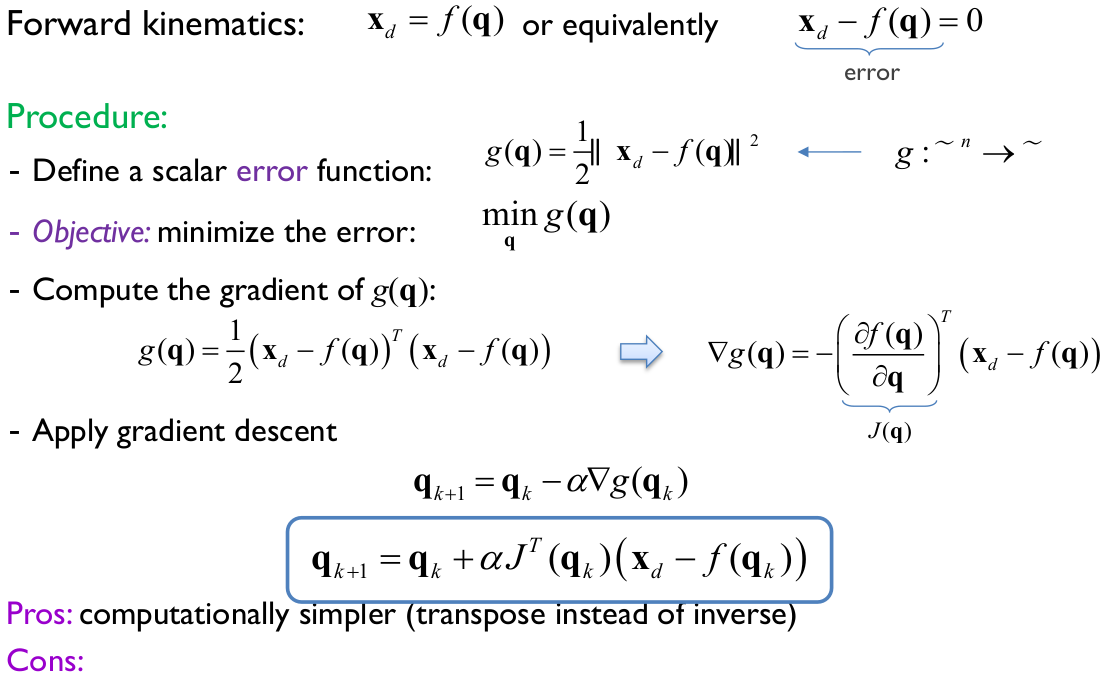
\includegraphics[width=11cm]{sections/imgs/23.png}
\end{center}
Example in slides.

\subsection{Numeric computation of the Jacobian}
For complex robots it is tedious to compute the Jacobian numerically.\\
\textbf{Solution:} Numeric differentiation

\begin{center}
	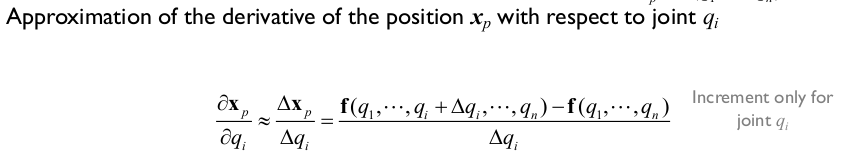
\includegraphics[width=12cm]{sections/imgs/24.png}\\
	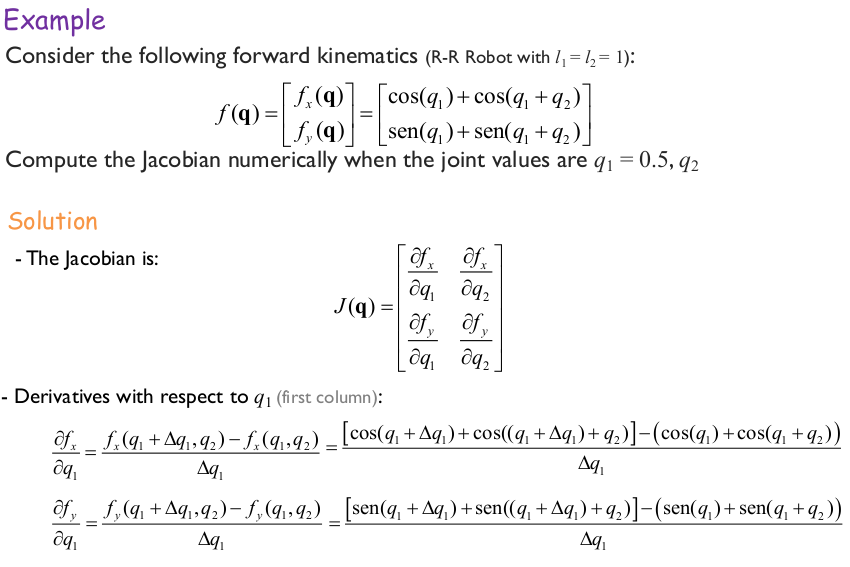
\includegraphics[width=12cm]{sections/imgs/25.png}\\
	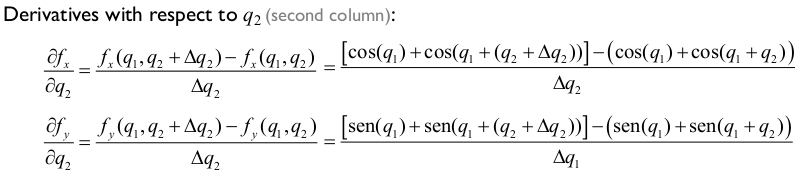
\includegraphics[width=12cm]{sections/imgs/26.png}\\
	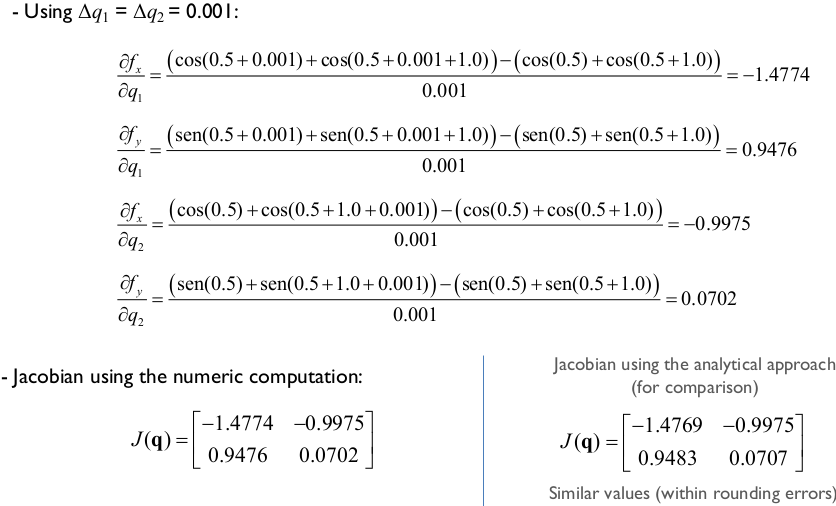
\includegraphics[width=12cm]{sections/imgs/28.png}	
\end{center}


\section{Jacobi Matrix (``Jacobian'')}

The Jacobian is the generalization of the differentiation to multi-dimensional functions, and contains all partial derivatives of function $ f $`s components, namely $ f_1 , f_2 , ..., f_{m} $ w.r.t its $ n $ parameters:

\begin{center}
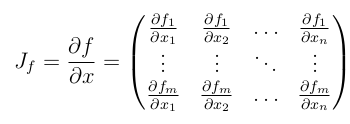
\includegraphics[width=7cm]{sections/imgs/39.png}
\end{center}
Example:
\begin{center}
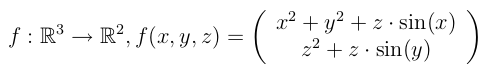
\includegraphics[width=7cm]{sections/imgs/40.png}
\includegraphics[width=7cm]{sections/imgs/41.png}
\end{center}

\subsection{Applications in Mathematics}
\subsubsection{Taylor's theorem}
One important usage of the Jacobian is the approximation of a function f in a sufficiently small neighborhood about a point $ x \in \mathbb{R}^{n} $, known as Taylor’s theorem:
\[ f (x + \delta x) \approx f (x) + \frac{\partial f}{\partial x} \cdot \delta x =  f (x) + \mathbf{J}_{f} (x) \cdot \delta x \]

\subsubsection{Multi-dimensional chain rule}
\[ (f \circ g)^{'} (t) = f^{'} (g (t)) g^{'} (t) \] 

The scalar derivatives are being replaced with Jacobi matrices: 
\[\mathbf{J_{a}} (f \circ g) = \mathbf{J}_{g (\mathbf{a})} (f) \mathbf{J_{a}} (g), \quad \mathbf{a} = (x,y,z)^T \]

\subsection{Jacobian as the Derivative of the Position Representation (Differential motion)}
We're often not only interested in position and orientation themselves, but also how they are affected by changes in robot parameters $\delta \theta$. These changes can be either small changes (leading to approximation via Taylor’s theorem), or velocities (specified as derivatives of a joint trajectory).

\begin{center}
	\includegraphics[width=6cm]{sections/imgs/4_pos_velocities.png}
\end{center}
We assume that we are given a position description of a robot coordinate system in form of a function $f$ (params: joint positions, mapped to 6-dim position and orientation representation). Because this representation could use quaternions, rotation matrices or variants of Euler angle conventions, this leads to different Jacobians.

\begin{center}
	$f: \mathbb{R}^{n} \rightarrow \mathbb{R}^{6}, (x_1 , x_2 , ..., x_{n} \mapsto (y_1 , y_2 ,...,y_{6} ))$
\end{center}

We define joint coordinates $q_i$, which combine revolute and prismatic joints. Then, the Jacobian is obtained from the derivative of the position representation w.r.t. the joint coordinate vector $\frac{\partial f(q)}{\partial q}$.

\begin{center}
	\includegraphics[width=6cm]{sections/imgs/4_joint_coordinates.png}
	\includegraphics[width=7cm]{sections/imgs/4_direct_diff.png}
\end{center}

An example from the Stanford Lecture:

\begin{center}
	\includegraphics[width=10cm]{sections/imgs/4_position_derivative_example.png}
\end{center}

\textbf{Note that in the TUM lecture material, the joint coordinates are denoted as $\Theta$}. Since the joint angles of a robot must vary over time to cause a motion, the joint positions $ \Theta_{1} , \Theta_{2} , ..., \Theta_{n} $ depend on time $ t $. However, we usually omit the $t$ in $ \Theta_{i} (t) $. All in all:

\[ \Theta (t): \mathbb{R} \rightarrow \mathbb{R}^{n}, t \mapsto (\Theta_{1} (t)  , \Theta_{2} (t)  , ..., \Theta_{n} (t))^T  \]

Then, the position representation at time $ t $ is written as follows:
\[ f (\Theta (t)), \qquad \mathbb{R} \rightarrow \mathbb{R}^{6}\]

\subsubsection{Craig's derivation of rotational velocities}
He uses a rotation-vector $ \boldsymbol{v} \in \mathbb{R}^{3} $ that represents the axis of rotation through its direction and the angle of rotation through its length $ \left| \boldsymbol{v} \right| $. The $\boldsymbol{0}$ vector represents the identity.

Differentiating rotation vectors $ \boldsymbol{v} $ w.r.t joint angles leads exactly to the angular velocity vectors $ \boldsymbol{\omega} $ that are used in his book.
 
\subsection{Jacobians and Velocities}
The Jacobian has the nice property of defining a relation between linear and angular velocities in joint space and velocities in cartesian space (for example of the end-effector). Here, we are interested in derivative of the position representation $ f $ w.r.t. time. 

In analogy to the position representation with small changes in the link coordinates, the same Jacobian connects the derivative of the position representation w.r.t. time and the angular and linear velocities of the joint coordinates:

\begin{center}
	\includegraphics[width=3.5cm]{sections/imgs/4_velocity_derivative.png}\\
\end{center}

The proof written in the notation of the TUM lecture (the first line applies the chain rule):
\begin{align*}
	 \dot{f} = \frac{\partial f}{\partial t} &= \frac{\partial f}{\partial (x_1 , ..., x_{n})} \frac{\partial \Theta}{\partial t} \\
								   &= \frac{\partial f}{\partial (x_1 , ..., x_{n})} \left( \frac{\partial \Theta_1}{\partial t} , \frac{\partial \Theta_{2} }{\partial t},..., \frac{\partial \Theta_{n}}{\partial t} \right)^T \\
								   &= J \cdot \dot{\Theta}
\end{align*}

The individual components of $f$ are the derivative the the position $\dot{x}_P$ and of the orientation $\dot{x}_R$ and are related to the joint coordinates by individual Jacobians:

\begin{center}
	$\left[\begin{array}{c}
	\dot{x}_P \\
	\dot{x}_R \\
	\end{array}\right]_{6 \times 1}=\left[\begin{array}{l}
J_{x_P} \\
J_{x_R}
\end{array}\right]_{6 \times n} \left[\begin{array}{c}
	\dot{\Theta}_{1} \\
	... \\
	\dot{\Theta}_{n}
	\end{array}\right]_{n \times 1}=J_{6 \times n}\left[\begin{array}{c}
	\dot{\Theta}_{1} \\
	... \\
	\dot{\Theta}_{n}
	\end{array}\right]_{n \times 1}$
\end{center}

Keep in mind that the Jacobian depends on the following circumstances:
 \begin{itemize}
	\item How are positions/orientations represented? A Jacobian that is based on cartesian coordinates will look different than one based on Euler angles. This following images shows the possible representations of position and orientation:
	\[\centering \includegraphics[width=4cm]{sections/imgs/4_X_pos_orientations.png}\]
	\item What is the reference coordinate system for the Jacobian?
	\item How is the current joint configuration?
 \end{itemize}

\textit{Note that for this reason, the Stanford Lecture distinguishes between a Jacobian $J_x$ for the particular representation used in $X$ and a basic Jacobian $J_0$.} These two matrices are related by a matrix $E$ that relates the linear velocity to the position representation and the angular velocity to the orientation representation.

\begin{center}
	$\begin{aligned}
&\dot{x}_{P}=E_{P}\left(x_{P}\right) v \\
&\dot{x}_{R}=E_{R}\left(x_{R}\right) \omega
\end{aligned}$
\end{center}

Herein, $\dot{x}_{P}$ and $\dot{x}_{R}$ are the derivatives of $f$ w.r.t. time and and $v$ and $\omega$ are the linear and angular velocity (these do not match $\dot{x}_{P}$ and $\dot{x}_{R}$ for certain representations!). The following figure shows how the Jacobian and the basic Jacobian are related:

\begin{center}
	\includegraphics[width=7cm]{sections/imgs/4_jacobian_and_basic_jacobian.png}
	\includegraphics[width=8cm]{sections/imgs/4_x_basic_jacobian_relation.png}
\end{center}

Usually, we want to know $v$ and $\omega$ and derive them from the third equation on the right side of the figure above.

 
\subsection{Velocities}

Linear velocities are always measured in a specific coordinate frame, e.g. the velocity of point $p$ measured in frame $\{A\}$ w.r.t. frame $\{B\}$:

\begin{center}
	\includegraphics[width=6cm]{sections/imgs/4_linear_velocity.png}
	\includegraphics[width=6cm]{sections/imgs/4_pure_translation.png}
\end{center}

The linear velocity from rotational motion derives from the cross product of the angular velocity with the points vector, as seen in the left figure below. When combining linear and angular velocities, one must make sure to express them w.r.t. the correct coordinate frame, hence the right figure.

\begin{center}
	\includegraphics[width=7cm]{sections/imgs/4_rotational_motion.png}
	\includegraphics[width=8cm]{sections/imgs/4_sim_lin_and_angular_motion.png}
\end{center}

With these concepts, the angular and linear velocities in robot joints are propagated from the base frame to the end-effector frame.

\begin{minipage}[c]{0.5\textwidth}
$
\begin{aligned}
	&\ {}^{i+1} v_{i+1} = {}^{i+1}_{i} R ({}^{i} v_{i} + {}^{i} \omega_{i} \times {}^{i} P_{i+1}) + \dot{d}_{i+1} \cdot {}^{i+1} \hat{Z}_{i+1}\\
	&\ {}^{i+1} \omega_{i+1} = {}^{i+1}_{i} R \cdot {}^{i} \omega_{i} + \dot{\Theta}_{i+1} \cdot {}^{i+1} \hat{Z}_{i+1}\\
\end{aligned}
$
\begin{center}
	$\dot{d}_{i+1}$ or $\dot{\Theta}_{i+1}$ for prismatic/ revolute joints (scalars).
\end{center}

\end{minipage}
\hfill
\begin{minipage}[c]{0.5\textwidth}
\includegraphics[width=9cm]{sections/imgs/4_velocity_propagation.png}\end{minipage}

The linear velocity w.r.t. frame $i+1$ is the sum of the linear velocity of frame $i$, the cross product of the angular velocity of frame $i$ with the distance between the two frames and the joint velocity along $\hat Z_{i+1}$ if $i+1$ is a prismatic joint (otherwise, $\dot{d}_{i+1}=0$). ${}^{i+1}_{i} R$ maps the vectors from from $i$ to frame $i+1$.\\
The angular velocity w.r.t. frame $i+1$ is composed of the  angular velocity of of the previous frame plus the angular velocity around $\hat Z_{i+1}$ if $i+1$ is a revolute joint.\\

The expressions for the linear and angular velocities at a given frame $n$ can be used to determine the full Jacobian indirectly:
\[ {}^{n} J \dot{\Theta} = \begin{pmatrix} {}^{n} v_n \\ {}^{n} \omega_{n} \end{pmatrix} \]
where the shape of the Jacobian on the left hand side can be determined from the shape of the linear-angular velocity vector on the right hand side (by factoring out the derivatives of the joint coordinates). Herein, the expressions for ${}^{n} v_n$ and ${}^{n} \omega_{n}$ are obtained from the two equations above.

An example for this is found in \href{https://youtu.be/fwHc0a8DMQ0?t=4040}{Lecture 6 of the Stanford course}.

\subsection{Explicit Form}

This section details how one can easily \textit{see} the Jacobian matrix in a manipulator. The next figure shows a manipulator with prismatic and revolute joints:
\\

\begin{minipage}[c]{0.5\textwidth}
	\includegraphics[width=9cm]{sections/imgs/4_jacobian_explicit_form.png} 
\end{minipage}
\hfill
\begin{minipage}[c]{0.5\textwidth}
	\begin{center}
	\begin{enumerate}
		\item The impact of each joint type on the end-effector is given in the table.
		\item The linear/ angular velocity of prismatic/ revolute joints is a function of the joints' $Z_i$ axes and joint coordinates $q_i$ ($\dot d$ or $\dot \theta$).
		\item The total velocities at the end-effector are the sum over the components from all joints.
	\end{enumerate}
	\end{center}
\end{minipage}
\\

In order to derive the Jacobian, we need to factor out the $q$s:\\

\begin{minipage}[c]{0.5\textwidth}
	\includegraphics[width=9cm]{sections/imgs/4_jacobian_explicit_form_2.png}
\end{minipage}
\hfill
\begin{minipage}[c]{0.5\textwidth}
	\begin{center}
	\begin{enumerate}
		\item Linear velocity: Each column in $J_v$ is the joint axis if the joint is prismatic or the cross product of the axis with the vector connecting the joint to the end-effector if the joint is revolute.
		\item Angular velocity: Each column in $J_\omega$ is the  joint axis if the joint is revolute or the $\boldsymbol{0}$ vector if it is prismatic.
		\item \textit{Note:} We need to express all vectors w.r.t. the frame in which we want to define our Jacobian.
	\end{enumerate}
	\end{center}
\end{minipage}\\

When using cartesian coordinates, we can also obtain $J_v$ directly from the derivative of the forward kinematics (or ``translation'' column in the homogeneous transform) w.r.t. the joint coordinates $q$. This is clearer when looking at the left side of the next figure. \\

The full Jacobian $J$ in some frame then consists of these $J_v$ and $J_\omega$ matrices. In order to express $J$ in reference frame $\{0\}$ we need to multiply every $Z_i$ axis with the the respective mapping ${}^0_i R$, as shown in the next figure. Note that the product ${}^0_i R \ Z_i$ is simply the third column of the rotation matrix! If we have the homogeneous transform, we can just pick the components for our Jacobian!\\

\begin{center}
	\includegraphics[width=8cm]{sections/imgs/4_jacobian_in_a_frame.png}
	\hfill
	\includegraphics[width=8cm]{sections/imgs/4_J_in_frame_0.png}
\end{center}

In \href{https://youtu.be/6SRTAoyzC6A?t=2235}{lecture 7 of the Stanford Lecture} you can find an example to practice \textit{seeing} the Jacobian.

Finally, these two rules may help (derived in Lecture 8 of the Stanford lecture):
\begin{center}
	\includegraphics[width=6cm]{sections/imgs/4_jacobian_relate_frames.png}
\end{center}

\subsection{Kinematic Singularity}

If the configuration of the robot manipulator reaches a singularity, the end-effector \textit{locally} loses the ability to move in a direction or to rotate about a direction, e.g. because two axes of revolute joints become collinear (see \href{https://youtu.be/XrNdB4k5kUk?t=575}{this explanation}).

Since the singularity happens, when $Z$ axes are aligned, the Jacobian does not have full rank in these situations (columns become dependant). In this case, the determinant is zero.
\begin{center}
	$
	\begin{aligned}
		 \det(J)&=0 \\
		 \det({}^i J)&=\det({}^j J)\\
		 \det(J)&=\det(J^T J)\ \text{   Trick if $J$ is not square.}
	\end{aligned}
	$
\end{center}
The determinant is the same in every reference frame! We can then find all singular configurations by setting the $\det(J)$ in any reference frame to zero.\\

\begin{minipage}[c]{0.5\textwidth}
	\includegraphics[width=8cm]{sections/imgs/4_kinematic_singularities.png}
\end{minipage}
\hfill
\begin{minipage}[c]{0.5\textwidth}
	\begin{center}
	\begin{enumerate}
		\item When the second joint angle is zero ($\theta_2=0$), the Jacobian in this frame becomes rank 1.
		\item From the relationship $[\delta x, \delta y]^T = J \ \delta\Theta$ follows that no motion in the local $x$ direction is possible. This is a singularity.
	\end{enumerate}
	\end{center}
\end{minipage}\\

\subsection{Jacobian for Approximating very small (``infinitesimal'') Movements}
Taylor's theorem (which states that a function behaves like its derivative in a sufficiently small environment) can be used to approximate how the position of the end effector changes whenever small changes are made to robot parameters. 

The theorem can be used to derive the following: 
\[ \delta x \approx J^{-1} (f (x + \delta x) - f (x))  \]
$ \delta x $ denotes a small change in $ x $, or a small change in the robot parameters. Using this equation, we can relate small changes $ \delta x $ in joint parameters to a small change $ f (x+ \delta x) - f (x) $ in position, and vice-versa.

This is the reason why singular configurations should be avoided: $ J $ becomes ill-conditioned near those, meaning that computed $ \delta x $ might approach infinity.

Singular positions are reached when $ det(J) = 0 $. Using this condition, we can figure out which joint parameters should be avoided.

\subsection{Frame of reference of a Jacobian}
Given a Jacobian in reference system B, the following equation related joint velocities to cartesian and angular velocities.
\[ \begin{pmatrix} {}^{B} v\\ {}^{B} \omega \end{pmatrix} = {}^{B} J (\Theta) \dot{\Theta}\]
And for a Jacobian w.r.t system A:
\[ {}^{A} J (\Theta) \dot{\Theta } = 
	\begin{pmatrix} {}^A_B R & \mathbf{0} \\ \mathbf{0} & {}^A_B R \end{pmatrix} {}^B J (\Theta) \dot{\Theta} \quad \Rightarrow \quad {}^A J (\Theta ) = \begin{pmatrix} {}^A_B R & \mathbf{0} \\ \mathbf{0} & {}^A_B R \end{pmatrix} {}^B J (\Theta)  \]

\subsection{Forces and Torques in Static Manipulators}
This section is based on page 156 of the book, exercise sheet 3 and the 8th lecture of the Stanford course.

In the figure below, two fundamental relations between torque exerted through motion around an axis and the force at a given point are derived.

\begin{center}
	\includegraphics[width=9cm]{sections/imgs/4_force_torque.png}
\end{center}

The linear velocity $v$ is the cross product between $\omega$ and the point vector. $\omega \times p = - p \times \omega$ can be rewritten using the matrix operator $\hat{p}$ that expresses the cross product. In the right part of the figure we use the fact that $\hat{p} = (-\hat{p})^T$. When we calculate the results of the cross products, we are left with the equations in red. It turns out that, while linear and angular velocity are related via the Jacobian, torque is related to force via its transpose.\\

The book derives this equation in another way: in the multidimensional case, work is the dot product of a vector force or torque and a vector displacement:
\[ \mathcal{F} \cdot \delta \mathcal{X} = \tau \cdot \delta \Theta  \]
where $ \mathcal{F} $ is a $6\times1$ cartesian force-moment vector acting at the end-effector, $ \delta \mathcal{X} $ is a $6\times1$ infinitesimal cartesian displacement of the end-effector, $ \tau $ is a $6\times1$ vector of torques at the joints, and $ \delta \Theta $ is a $6\times1$ vector of infinitesimal joint displacements. 

\begin{center}
	$\left(\begin{array}{c}
\tau_{1} \\
\tau_{2} \\
\vdots \\
\tau_{n}
\end{array}\right)=\tau={ }^{A} J^{T A} \mathcal{F}={ }^{A} J^{T}\left(\begin{array}{c}
{}^{A}f \\
{}^{A}n
\end{array}\right)$
\end{center}

The Jacobian transpose maps cartesian forces acting at the hand into equivalent joint torques. When the Jacobian is written with respect to frame $\{0\}$, then force vectors written in $\{0\}$ can be transformed, as follows:
\[ \tau = {}^0 J^T \ {}^0\mathcal{F} \]

If we calculate the static equilibrium for each link in a robot manipulator, we are able to relate the forces and torques at the end effector to the forces and torques at the base. The next figure shows the (reaction) forces $f$ and torques $n$ in each link of the manipulator on the left and the static equilibrium of one link on the right.
\begin{center}
	\includegraphics[width=7cm]{sections/imgs/4_propagate_forces_2.png}
	\hfill
	\includegraphics[width=9cm]{sections/imgs/4_propagate_forces.png}
\end{center}

We can then propagate the forces $f_i$ and torques $n_i$ acting on each link from the end-effector to the base:

\begin{center}
	$\begin{aligned}
	&{ }^{i} f_{i}={ }_{i+1}^{i} R \cdot{ }^{i+1} f_{i+1} \\
	&{ }^{i} n_{i}={ }_{i+1}^{i} R \cdot{ }^{i+1} n_{i+1}+{ }^{i} P_{i+1} \times{ }^{i} f_{i}
	\end{aligned}$
\end{center}

The torque that is exerted on prismatic/ revolute joins is given from the projection (inner product) on the joint axis, as shown in the next figure:

\begin{minipage}[c]{0.5\textwidth}
	\includegraphics[width=8cm]{sections/imgs/4_prismatic_revolute_torque.png}
\end{minipage}
\hfill
\begin{minipage}[c]{0.5\textwidth}
\begin{center}
$\begin{aligned}
&\tau_{i}={ }^{i} n_{i}^{\mathrm{T} i} Z_{i}={ }^{i} n_{i}^{\mathrm{T}}\left(\begin{array}{l}
0 \\
0 \\
1
\end{array}\right) \\
&\tau_{i}={ }^{i} f_{i}^{\mathrm{T} i} Z_{i}={ }^{i} f_{i}^{\mathrm{T}}\left(\begin{array}{l}
0 \\
0 \\
1
\end{array}\right)
\end{aligned}$
\end{center}

\end{minipage}

The quantities $\tau_i$ thus specify the amount of torque resp. force that is affecting the joint, and thus the amount of torque resp. force that the robot should counteract in order to remain static. The joint torques/forces $\tau_i$ are 1-dimensional quantities.


\newpage
\section{Robot Dynamics}

The field of analytical dynamics, or more briefly dynamics, is concerned with the relationship between motion of bodies and its causes, namely the forces acting on the bodies and the properties of the bodies (particularly mass and moment of inertia) influencing that movement. This is in contrast to kinematics, where we were not concerned with the physical phenomena causing robot movement, but only with the movement itself.

We want to come up with equations of motion for any nDOF system, which express the force require to cause motion. The expression should have the form $ \dot{q} = f (q,t)$\\
We can use it to choose an appropriate controller that will put our dynamical system in a desired state.
This section is based on \href{https://www.youtube.com/watch?v=o3Xx3vi6qzo&list=PL65CC0384A1798ADF&index=12}{Lecture 11} and covered in exercise 4.

\subsection{Rigid Body Dynamics}
\begin{center}
	\includegraphics[width=14cm]{sections/imgs/29.png}
\end{center}

\subsection{Newton-Euler Method}
Overall, the purpose of the Newton-Euler-Method is determining the joint torques $\tau$ that are required to achieve a desired motion of the robot. More specifically, if we have a joint trajectory $\Theta (t)$ that describes the positions and velocities for a certain trajectory of the robot, then the Newton-Euler method will allow us to compute corresponding $\tau (t)$ that will, in an ideal world (no friction or other disturbances for the moving robot), cause the robot to carry out the desired trajectory.

\subsubsection{Newton's equation}
A rigid body's center of mass is accelerating with $ \dot{v}_{c} $ when the force $ F $ acts on it. The acceleration is given by
\[ F = m \dot{v}_{c} \]
\begin{center}
	\includegraphics[width=6cm]{sections/imgs/36.png}
\end{center}

\subsubsection{Euler's equation}
The rigid body in the image below rotates with angular velocity $ \omega $ and with angular acceleration $ \dot{ \omega} $. Then, the moment $ N $, which acts on the link is:
 \[ N = {}^{C} I \dot{\omega } + \omega \times {}^{C} I \omega \]
where $ {}^{C} I $ is the inertia tensor that is computed with respect to the center of mass in frame $C$, a $3\times3$ matrix that describes the distribution of masses in a link. \begin{center}
	\includegraphics[width=6cm]{sections/imgs/37.png}
\end{center}

\subsubsection{Linear acceleration}
The linear acceleration is the derivative of the linear velocity of the joint w.r.t. time. In case of a rotational joint $i+1$, we have:
\begin{center}
$\begin{aligned}
{}^{i+1} v_{i+1} &= {}^{i+1}_{i} R ({}^{i} v_{i} + {}^{i} \omega_{i} \times {}^{i} P_{i+1})\\
{ }^{i+1} \dot{v}_{i+1}&={ }_{i}^{i+1} R\left({ }^{i} \dot{\omega}_{i} \times{ }^{i} P_{i+1}+{ }^{i} \omega_{i} \times\left({ }^{i} \omega_{i} \times{ }^{i} P_{i+1}\right)+{ }^{i} \dot{v}_{i}\right)
\end{aligned}$
\end{center}

When joint $i+1$ is prismatic, the formula becomes more complicated:

\begin{center}
$\begin{aligned}
{}^{i+1} v_{i+1} &= {}^{i+1}_{i} R ({}^{i} v_{i} + {}^{i} \omega_{i} \times {}^{i} P_{i+1}) + \dot{d}_{i+1} \cdot {}^{i+1} \hat{Z}_{i+1} \\
{ }^{i+1} \dot{v}_{i+1}&={ }_{i}^{i+1} R\left({ }^{i} \dot{\omega}_{i} \times{ }^{i} P_{i+1}+{ }^{i} \omega_{i} \times\left({ }^{i} \omega_{i} \times{ }^{i} P_{i+1}\right)+{ }^{i} \dot{v}_{i}\right)+2 \cdot{ }^{i+1} \omega_{i+1} \times \dot{d}_{i+1}{ }^{i+1} Z_{i+1}+\ddot{d}_{i+1}{ }^{i+1} Z_{i+1}
\end{aligned}$
\end{center}

\subsubsection{Angular acceleration}
The angular velocities and accelerations for rotational joints are:
\begin{center}
$\begin{aligned}
{ }^{i+1} \omega_{i+1} &={ }_{i}^{i+1} R \cdot{ }^{i} \omega_{i}+\dot{\Theta}_{i+1} \cdot{ }^{i+1} Z_{i+1} \\
{ }^{i+1} \dot{\omega}_{i+1} &={ }_{i}^{i+1} R \cdot{ }^{i} \dot{\omega}_{i}+{ }_{i}^{i+1} R \cdot{ }^{i} \omega_{i} \times \dot{\Theta}_{i+1} \cdot{ }^{i+1} Z_{i+1}+\ddot{\Theta}_{i+1}{ }^{i+1} Z_{i+1}
\end{aligned}$
\end{center}

When joint $i+1$ is prismatic, the formulas simplifies to:

\begin{center}
$\begin{aligned}
&{ }^{i+1} \omega_{i+1}={ }_{i}^{i+1} R \cdot{ }^{i} \omega_{i}\\
&{ }^{i+1} \dot{\omega}_{i+1}={ }_{i}^{i+1} R \cdot{ }^{i} \dot{\omega}_{i}
\end{aligned}$
\end{center}

\subsubsection{Newton-Euler Algorithm}
Each link of a manipulator is considered as a rigid body. Remember the recursive equations for the forces and torques propagated to the next link from the previous chapter? In the non-static scenario, we need to modify them, such that they regard the velocities and accelerations acting on each link.

The Newton-Euler-Method is composed of two phases: A forward phase and a backwards phase. In the first phase, the velocities and accelerations (both rotational and linear) are computed for each joint. Using these values, we compute the forces and torques that the motion exerts on each link. In the backwards phase, these forces and torques are used to compute the forces and torques that act on each joint.

 The linear velocity of the center of mass for rotational and prismatic joints is:

\begin{center}
	${ }^{i} \dot{v}_{C_{i}}={ }^{i} \dot{\omega}_{i} \times{ }^{i} P_{C_{i}}+{ }^{i} \omega_{i} \times\left({ }^{i} \omega_{i} \times{ }^{i} P_{C_{i}}\right)+{ }^{i} \dot{v}_{i}$
\end{center}

In the next step, we can compute the forces and torques that apply to the center of mass of each link from the accelerations and speeds that we have just computed:

\begin{center}
$\begin{aligned}
{ }^{i} F_{i} &=m_i \cdot{ }^{i} \dot{v}_{C_{i}} \\
{ }^{i} N_{i} &={ }^{C_{i}} I_{i} \cdot{ }^{i} \dot{\omega}_{i}+{ }^{i} \omega_{i} \times{ }^{C_{i}} I_{i} \cdot{ }^{i} \omega_{i}
\end{aligned}$
\end{center}

Based on those forces and moments, we can compute $f_i$ and $n_i$ for joint $i$ of the manipulator:

\begin{center}
	$\begin{aligned}
		{ }^{i} f_{i} &={ }_{i+1}^{i} R \cdot{ }^{i+1} f_{i+1}+{ }^{i} F_{i} \\
		{ }^{i} n_{i} &={ }^{i} N_{i}+{ }_{i+1}^{i} R \cdot{ }^{i+1} n_{i+1}+{ }^{i} P_{C_{i}} \times{ }^{i} F_{i}+{ }^{i} P_{i+1} \times{ }_{i+1}^{i} R^{i+1} f_{i+1}
	\end{aligned}$
\end{center}

As in the static case, the values of $\tau_i$, compute as $\tau_i = {}^in^T_i \cdot {}^iZ_i$ for a rotational joint and $\tau_i = {}^if^T_i \cdot {}^iZ_i$ for a translational joint.

\begin{center}
	\includegraphics[width=8cm]{sections/imgs/6_newton_euler_recursive_eq.png}
	\hfill
	\includegraphics[width=7cm]{sections/imgs/6_newton_euler_alg.png}
\end{center}

If we know the location of the center of mass and the inertia tensor of the link, then its mass
distribution is completely characterised. In order to move the links, we must
We accelerate and decelerate them. The forces required for such motion are a function
of the acceleration desired and of the mass distribution of the links. 

Newton's equation, along with its rotational analog, Euler's equation, describes how forces, inertias, and accelerations relate.

Exercise sheet 4 has a simple examples which demonstrates the Newton-Euler-Algorithm quite well.

\subsection{State-Space equation (M-V-G-form)}

We also need to take into account the effect of gravity on the links of the robot. This can be done by setting ${ }^{0} \dot{v}_{0}=-G$ where $G$ is the gravitational acceleration. We obtain the M-V-G-form by rearranging the equations of movement for the joint torques:

\begin{center}
	$\tau=M(\Theta) \ddot{\Theta}+V(\Theta, \dot{\Theta})+G(\Theta)$
\end{center}

$M$ is a $n\times n$ matrix, and $V$ as well as $G$ are $n\times 1$ vectors. Note that in general, $M$, $V$, $G$ are complex-valued. The matrix $M$ can be determined from the dynamics equations by factorizing all summands that contain  ̈$\ddot{\theta}$. Similarily, $V$ is determined by factorizing all summands that contain $\dot{\theta}$. Finally, $G$ is determined by factorizing all summands that contain $g$. $V$ can be further decomposed into components $B$ and $C$, yielding the configuration-space equation (or M-B-C-G-form):

\begin{center}
	$\tau=M(\Theta) \ddot{\Theta}+B(\Theta)[\dot{\Theta} \dot{\Theta}]+C(\Theta)\left[\dot{\Theta}^{2}\right]+G(\Theta)$
\end{center}

$B(\Theta)$ is a matrix of dimension $n \times n(n-1) / 2$, and $[\dot{\Theta} \dot{\Theta}]$ is an abbreviation for the vector

\begin{center}
	$\left(\dot{\Theta}_{1} \dot{\Theta}_{2}, \dot{\Theta}_{1} \dot{\Theta}_{3}, \ldots, \dot{\Theta}_{n-1} \dot{\Theta}_{n}\right)$
\end{center}

that has length $n(n-1) / 2$. This also explains the dimension of $B$: $n(n-1) / 2$ is the number of products $\Theta_{i} \Theta_{j}$ with $i \neq j$. The matrix $C$ has dimension $n \times n$, and $\left[\dot{\Theta}^{2}\right]$ in an abbreviation for the vector
\begin{center}
$$\left(\dot{\Theta}_{1}^{2}, \dot{\Theta}_{2}^{2}, \ldots, \dot{\Theta}_{n}^{2}\right)^{\mathrm{T}}$$
\end{center}

with length $n$. The matrices $B$ and $C$ can be determined by finding the coefficients of $\Theta_{i} \Theta_{j}$ and $\Theta_{i}^{2}$, respectively.

\subsection{Mass distribution}
In systems with a single degree of freedom, we often talk about the mass of a rigid
body. In the case of rotational motion about a single axis, the notion of the moment
of inertia is a familiar one. 
\subsubsection{Linear Momentum}

The rate of change of the linear momentum for a particle with mass $m$ is equal to the applied force.

\begin{center}
$\begin{aligned}
	\frac{d}{d t}(m v) &= F \\
	\varphi &= mv
\end{aligned}$
\end{center}

\subsubsection{Angular Momentum}
...is the total moment of the momentum of a rigid body's constituting particles:
\[ H_c = \int\limits_{\mathcal{B}}^{} r \times x \mathop{d m} = {}^{A}\mathbf{I} \omega  \]

Angular momentum can be understood as the cross-product of the linear momentum $mv$ and a position vector $p$. This follows from the fact that the rate of change of the angular momentum is equal to the applied moment, hence the left image below. For a rigid body (right image), the total angular momentum $\phi$ is the sum of angular momentum for all particles. The velocity is written as $\omega \times p_i$ and the mass is the integral over the density multiplied by the volume.
\begin{center}
	\includegraphics[width=8cm]{sections/imgs/6_angular_momentum.png}
	\hfill
	\includegraphics[width=8cm]{sections/imgs/6_rigid_body_angular_momentum.png}
\end{center}

Using the reformulation of the cross-product operator $\mathbf{\hat{p}}=\mathbf{p}\times$ and the fact that $\mathbf{\omega}\times\mathbf{p}=-\mathbf{p}\times\mathbf{\omega}$, wherein $\omega$ is shared among all points, we derive:

\begin{center}
$\begin{aligned}
	\mathbf{p} \times(\omega \times \mathbf{p})&=\hat{\mathbf{p}}(-\hat{\mathbf{p}}) \omega \\
	\phi &= \int_{V} p \times(\omega \times p) \rho d v = \left[\int_{V} -\hat{\mathbf{p}} \hat{\mathbf{p}} \rho d v\right] \omega = \mathbf{I}\omega \\
	\frac{d}{d t}(\mathbf{I} \omega)&=N
\end{aligned}$
\end{center}

\subsubsection{Inertia Tensor}

For a rigid body that is free to move in three dimensions, there are infinitely many possible rotation axes. In the case of rotation about an arbitrary axis, we need a complete way of characterizing the mass distribution of a rigid body. 

The \textbf{inertia tensor} can be
thought of as a generalization of the scalar moment of inertia of an object, relative to the frame attached to the object (rigid body). The left side of the following figure shows the derivation of the inertia tensor from the volume integral of $-\mathbf{\hat{p}}\mathbf{\hat{p}}$. Remember that $\hat{p}$ is the cross-product operator for a point on the rigid body relative to the origin. $I_{xx}, I_{yy}, I_{zz}$ are called \textit{moments of inertia}, while $I_{xy}, I_{xz}, I_{yz}$ are called \textit{products of inertia}.

\begin{center}
\begin{minipage}{0.5\textwidth}
	\begin{center}
		\includegraphics[width=8cm]{sections/imgs/6_inertia_tensor.png}
	\end{center}
\end{minipage}
\begin{minipage}{0.49\textwidth}
	\begin{tabular}{cc}
		\includegraphics[width=4cm]{sections/imgs/33.png}&\\
		\includegraphics[width=3.5cm]{sections/imgs/34.png}& \includegraphics[width=3cm]{sections/imgs/35.png}
	\end{tabular}
\end{minipage}
\end{center}

For an example, check example 6.1 on page 169 or 6.2 on page 171.

\textbf{Some properties:}
\begin{itemize}
	\item Inertia matrices are positive-definite, symmetric matrices.
	\item The inertia matrix is not in general constant and is frame-dependent:
		\[ \mathbf{I}_{c}^{i} = R_{i}^T \mathbf{I}_{c} R_{i} \]
	\item Any rigid body has a set of principal directions with respect to which the inertia matrix is diagonal.
	\item If $xy$ is the plane of symmetry, then $ I_{xz} = I_{yz} = 0 $ (similarly for $xz$ or $yz$).
	\item If the body is axissymmetric (e.g. symmetric about $z$), then the inertia matrix is diagonal and 2 of the moments of inertia equal (e.g. $ I_{xx} = I_{yy} $ if z is axis of symmetry)
\end{itemize}

\subsubsection{Parallel-Axis Theorem}
... is a way of computing how the inertia tensor changes under \textit{translations} of the reference coordinate system (s.t. the axes remain parallel). It relates the inertia tensor in a frame with origin at the center of mass ${}^CI$ to the inertia tensor with respect to another reference frame ${}^AI$. $C$ is located at the center of mass of the body, and $A$ is an arbitrarily translated frame. The theorem can be stated as:
\begin{align*} \label{eq:pat}
	{}^{A} I_{zz} &= {}^{C} I_{zz} + m (x_{c}^2 + y_{c}^2) \\
	{}^{A} I_{xy} &= {}^{C} I_{xy} - m x_{c} y_{c} 
\end{align*}
Where $ P_{c} = [x_{c} , y_{c} , z_{c}]^T $ locates the center of mass relative to $A$. The remaining moments and products of inertia are computed from permutations of $ x,y,z $. The theorem in vector-matrix form:
\[ {}^{A} I = {}^{C} I + m [P_{c}^T P_{c} I_{3} - P_{c} P_{c}^T] \]
with $ I_{3} $ as the identity matrix. The left side of the following image shows the new reference frame $A$ and the center of mass $m$, as well as the connecting vector $P_{c}$.

\begin{center}
\includegraphics[width=7cm]{sections/imgs/6_parallel_axes.png}
\hfill
\includegraphics[width=8cm]{sections/imgs/38.png}
\end{center}


\subsection{Euler-Lagrange Equations}

The Lagrangian dynamic formulation is another method for determining the dynamics of a robot which is derived from energy considerations. The Lagrange equation is:

\begin{center}
	$\frac{d}{dt} \frac{\partial L}{\partial \dot{\Theta}} - \frac{\partial L}{\partial \Theta} = \tau$
\end{center}

where the Lagrangian $L=k-u$ is the difference between the kinetic energy $k$ and the potential energy $u$. Since $U=U(\Theta)$, the equation simplifies to

\begin{center}
	$\tau=\frac{d}{d t} \frac{\partial k}{\partial \dot{\Theta}}-\frac{\partial k}{\partial \Theta}+\frac{\partial u}{\partial \Theta}$.
\end{center}

The derivatives of the Lagrange equation are given the left part of the figure below. We set $G=\frac{\partial u}{\partial \Theta}$ since it only depends on $\Theta$. By calculating the derivatives, we see that the Lagrange equation is in M-V-G-form. Next, we can identify $M(q)$ from the expression $k=\frac{1}{2} \dot{q}^{T} M \dot{q}$. With knowledge of $M$ the expression in pink gives us $V(q, \dot{q})$.
\\

\begin{minipage}[c]{0.5\textwidth}
	\includegraphics[width=9cm]{sections/imgs/6_lagrange_mvg.png}
\end{minipage}
\hfill
\begin{minipage}[c]{0.5\textwidth}
\begin{center}
	\includegraphics[width=6cm]{sections/imgs/6_lagrange_vmg_2.png}
\end{center}

\end{minipage}

For each link of the robot, the kinetic energy can be computed as (and is the same for any reference frame of the velocities):

\begin{center}
	$k_{i}=\frac{1}{2} m_{i} v_{C_{i}}^{\mathrm{T}} \cdot v_{C_{i}}+\frac{1}{2} {}^i \omega_{i}^{\mathrm{T}} \cdot{ }^{C_{i}} I_{i} \cdot{ }^{i} \omega_{i}$
\end{center}

The first term corresponds to the kinetic energy caused by the linear motion of the link, and the second term corresponds to the kinetic energy caused by the rotational velocity of the link. To determine these energies, we need to compute the linear and rotational velocities of the joints. The overall kinetic energy computes then as sum of the kinetic energies of all links:

\begin{center}
	$k=\sum_{i=1}^{n} k_{i}$
\end{center}

Another way to compute kinetic energy is

\begin{center}
	$k(\Theta, \dot{\Theta})=\frac{1}{2} \dot{\Theta}^{\mathrm{T}} M(\Theta) \dot{\Theta}$
\end{center}

where $M$ again is the $n\times n$ mass matrix from the M-V-G form of the dynamics equations. By setting both formulas for $k$ equal to each other and expressing the velocities at the centres of mass with their Jacobians, we derive an expression for $M$, as the next figure shows. Note that these Jacobians relate the joint parameters to the velocities at the centres of mass of each link instead of at the joints. As shown in the bottom right corner, they only regard these relations up to the link $i$. All columns after this point are zero.
\\

\begin{minipage}[c]{0.5\textwidth}
	\includegraphics[width=9cm]{sections/imgs/6_mass_matrix_jacobian.png}
\end{minipage}
\hfill
\begin{minipage}[c]{0.5\textwidth}
\begin{center}
	\includegraphics[width=7cm]{sections/imgs/6_mass_matrix_jacobian_2.png}
	\vfill
	\includegraphics[width=7cm]{sections/imgs/6_mass_matrix_jacobian_3.png}
\end{center}
\end{minipage}

To compute all energies that are present in this system, we also need to take into account the potential energy:

\begin{center}
	$u_{i}=-m_{i} \cdot{ }^{0} g^{\mathrm{T}} \cdot{ }^{0} P_{C_{i}}+u_{\mathrm{ref}_{i}}$
\end{center}

Here, $g$ is the vector of gravity, ${ }^{0} P_{C_{i}}$ denotes the centre of mass of link $i$, and $u_{\mathrm{ref}_{i}}$, is an arbitrary constant (the constant is added because potential energy depends on height, and a certain base height can be chosen arbitrarily). In the further computations, this constant will not play a role, since only the derivatives of the potential energy are considered - and any constant will vanish when differentiated. 
By differentiating the potential energy, we obtain the gravity vector $G$, which also contains the Jacobians. Thus, another way to think of the gravity vector is as the torque in each joint that is caused by a force pulling down on every link of the robot. This is shown in the right part of the figure below.

\begin{center}
	\includegraphics[width=8cm]{sections/imgs/6_lagrange_potential_energy.png}
	\hfill
	\includegraphics[width=7cm]{sections/imgs/6_lagrange_potential_energy_2.png}
\end{center}

The computation of $\tau$ is finally done through the following formula:

\begin{center}
	$\tau=\frac{d}{d t} \frac{\partial k}{\partial \dot{\Theta}}-\frac{\partial k}{\partial \Theta}+\frac{\partial u}{\partial \Theta}$
\end{center}

It is also possible to compute the joint torques τi on a per-joint basis, which is more practical in most cases. The formula then becomes:

\begin{center}
	$\tau_{i}=\frac{d}{d t} \frac{\partial k}{\partial \dot{\Theta}_{i}}-\frac{\partial k}{\partial \Theta_{i}}+\frac{\partial u}{\partial \Theta_{i}}$
\end{center}
\section{Control}

Being able to establish the dynamics equations of a robot is still not enough to make it carry out a desired trajectory. There are several disturbances in physical systems that cannot be modelled, which means that a controlling scheme is required to alleviate the influence of those disturbances. The following schematic gives an overview of a typical control architecture:

\begin{center}
	\includegraphics[width=8cm]{sections/imgs/7_control_architecture.png}
\end{center}

The value $r$ would be the desired state of the system. Computing the difference $e=y_{m}-r$ yields the error of the current state $y_{m}$ with respect to the desired state. The controller takes $e$ into account when generating control signals $u$, in order to correct any error introduced by disturbances.

This section is based on the explanations in exercise 5, \href{https://www.youtube.com/watch?v=5-k2RzfIgoU&list=PL65CC0384A1798ADF&index=14}{lecture 13} and \href{https://www.youtube.com/watch?v=U3diaQ-iU0I&list=PL65CC0384A1798ADF&index=16}{lecture 14}.

\subsection{Mass-Spring-Systems}

As a prerequisite to understanding the function of a PD controller, mass-spring-systems have been studied in the lecture. The importance of these systems lies in their connection to the behaviour of the error $e$ in control problems. We will later see that the error $e$ behaves like a mass-spring-system itself.

\begin{center}
	\includegraphics[width=4cm]{sections/imgs/7_mass_spring_system.png}
\end{center}

The dynamic equation of the mass-spring-system is:

\begin{center}
	$m \ddot{x}+b \dot{x}+k x=f$
\end{center}

where $m$ is the mass of the object, $b$ is the friction constant and $k$ is the spring constant. The deflection of the object from its resting position is  denoted by $x$. This equation is, in the context of control, also called the \textit{open-loop-equation}, since it does not take into account any feedback from the system (like, e.g., in the case of a robot, joint position measurements from sensors or such).

We distinguish three possible cases for the applied force $f$: Under-damping leads to oscillation of the system (spring stiffness dominates), while over-damping leads to slow convergence to the resting position (friction dominates). Critical damping leads to the fastest possible transition of the system to its resting configuration, avoiding both overdamping and underdamping (friction and stiffness are in balance).

\begin{center}
	\includegraphics[width=7cm]{sections/imgs/7_critically_damped.png}
\end{center}

\subsubsection{Solution of the Dynamic Equation (Position Control)}

How can we achieve critical damping? The force $f$ that we exert on the object must depend on friction and spring forces, and we can assume that it’s of the form $f=-k_{p} x-k_{v} \dot{x}$ (proportional-derivative-/ PD-control; the formula is derived \href{https://youtu.be/5-k2RzfIgoU?t=3514}{here in the lecture}). This yields the \textit{closed-loop equation}:

\begin{center}
	$m \ddot{x}+\left(b+k_{v}\right) \dot{x}+\left(k+k_{p}\right) x=0$
\end{center}

We are interested in controlling the movement of the body, so we are interested in determining the function $x(t)$, which means we need to solve the differential equation. This is done by solving the characteristic equation:

\begin{center}
$m s^{2}+\left(b+k_{v}\right) s+\left(k+k_{p}\right)=0$	
\end{center}

The solutions to this quadratic equation are given by the well-known formula
$$
s_{1,2}=\frac{-\left(b+k_{v}\right) \pm \sqrt{\left(b+k_{v}\right)^{2}-4 m\left(k+k_{p}\right)}}{2 m}=\frac{-b^{\prime} \pm \sqrt{b^{\prime 2}-4 m k^{\prime}}}{2 m} .
$$
It is then common to abbreviate $\left(b+k_{v}\right)$ as $b^{\prime}$ and $\left(k+k_{p}\right)$ as $k^{\prime}$. The solutions $s_{1}, s_{2}$ determine the trajectory $x(t)$ as follows:
$$
x(t)=c_{1} e^{s_{1} t}+c_{2} e^{s_{2} t}
$$

A special case is $s_{1}=s_{2} \in \mathbb{R}$. This case corresponds to critical damping of the system. Note that this can be achieved by choosing $b^{\prime}$ and $k^{\prime}$ such that $b^{\prime 2}-4 m k^{\prime}=0$, or $b^{\prime}=2 \sqrt{m k^{\prime}}$ (we can assume $b^{\prime}$ and $k^{\prime}$ to be positive). In the case of an oscillating system, the equations can also be stated in a different form:

\begin{center}
$s^{2}+2 \zeta \omega_{n} s+\omega_{n}^{2}=0$
\end{center}

with the ``damping ratio'' $\zeta$ and the ``natural frequency'' $\omega_{n}$
 
\begin{center}
$
\begin{aligned}
\zeta &=\frac{b^{\prime}}{2 \sqrt{k^{\prime} m}} \\
\omega_{n} &=\sqrt{\frac{k^{\prime}}{m}}.
\end{aligned}
$
\end{center}

Now, we design our PD-controller by setting $k_p$ and $k_v$, such that we achieve critical damping (see the experiments in \href{https://www.youtube.com/watch?v=U3diaQ-iU0I&list=PL65CC0384A1798ADF&index=16}{lecture 14} for an example). Herein, if the damping ratio $\zeta$ is too small, the joint oscillates and if it is too large, it is overdamped (reaches the goal state slower). Moreover, the natural frequency $\omega$ is limited by an upper bound, as explained in the next section. If this upper bound is exceeded, the motion becomes unstable.
\subsubsection{Resonance}

Until now, we assumed that all parts of the mechanic systems we observed do not deform at all. But in reality, components of robots have a finite stiffness, which means that they deform minimally under stress. This can lead to the undesired effect of resonance, which leads to deformations adding up until finally components may be damaged.

A simple possibility of taking the effect of resonance into account is through enforcing the following inequality:
$$
\omega_{n} \leq \frac{1}{2} \omega_{\text {res }}
$$
Here, $\omega_{\text {res }}$ is the so-called resonant frequency of the object. If this condition holds, we can be sure that no undesired resonances occur.

\subsubsection{Control Partitioning}

Until now, we have used the following simple rule to influence the behaviour of a mass-spring system:
$$
f=-k_{p} x-k_{v} \dot{x}
$$
Using this rule, we were able to achieve critical damping of a mass-spring system, choosing parameters $k^{\prime}$ and $b^{\prime}$ according to $b^{\prime}=2 \sqrt{m k^{\prime}}$. However, the choice of $b^{\prime}$ depends on $m$, which is acceptable for a simple mass-spring system, but makes things very complicated in more complex systems. Thus, we want to decouple the mass-dependent part from the equation, using an extended rule that reads as follows:
$$
f=\alpha f^{\prime}+\beta
$$
This equation is known as the \textit{model-based portion}. Through this rule, we want to achieve the following: Factors $\alpha$ and $\beta$ should be chosen such that the system, considering only $f^{\prime}$ as input, behaves like a unit mass, governed by the equation
$$
\ddot{x}=f^{\prime}
$$
Writing down the complete equation for the system, we obtain
$$
m \ddot{x}+b \dot{x}+k x=\alpha f^{\prime}+\beta .
$$

Now comes the interesting part: How should we choose $\alpha$ and $\beta$ in order to achieve the desired effect? Obviously, $\beta=b \dot{x}+k x$ and $\alpha=m$ must hold. Note that we are now able to influence the system directly through $f^{\prime}$. This is the decoupled open-loop equation. Again, be aware that for the simple case of a mass-spring system there is not much gained through rewriting the system like this, but for manipulating more complicated systems, the advantage is substantial.

Now, we move again from the open-loop form to the closed-loop form. Thus, let $f^{\prime}$ again depend on spring force and friction force, such that
$$
f^{\prime}=-k'_{p} x-k'_{v} \dot{x}
$$
with some new constants $k_{p}'$ and $k_{v}'$. The equation of motion becomes
$$
\ddot{x}+k'_{p} x+k'_{v} \dot{x}=0
$$
In particular, we see that now $k_{v}$ and $k_{p}$ are now independent of system parameters. The system will always be critically damped if $k_{v}'=2 \sqrt{k'_{p}}$.

In other words, we want to approximate the mass-spring system with a unit mass system that is linearly scaled by $\alpha$ and $\beta$. Herein, $\alpha$ compensates for the mass ($m$ or the mass matrix $M$) and $\beta$ compensates for $b\dot x+kx$ (or other terms like centrifugal, coreolis and gravitational forces with $V$ and $G$). All terms that depend on $m$ cancel out and we are left with the equation for the unit mass system, for which we then design $k'_{v}$ and $k'_{p}$ independent of the mass.
\\

\begin{minipage}[c]{0.45\textwidth}
	\includegraphics[width=7cm]{sections/imgs/7_control_partitioning.png}
\end{minipage}
\hfill
\begin{minipage}[c]{0.45\textwidth}
In the slide on the left, the non-linear system $m\ddot x+b(x,\dot x)=f$ is approximated (through control partitioning) with the factors $\alpha$ and $\beta$. This equation is equivalent to $f'=\ddot x$ (the other terms cancel out), which is the unit mass system. The control loop shows how the unit mass system is linearly scaled with the factor $\hat m$ and $\hat b(x, \dot x)$.
\end{minipage}

\subsubsection{Trajectory following/ Motion Control}

Now we no longer assume that we are simply interested in achieving critical damping of a mass-spring system, but instead we want the system to carry out a certain trajectory. The computed trajectory shall be denoted by $x_{d}(t)$, and we assume that $x_{d}(t)$ is a twice continuously differentiable function. Let $e(t)=x_{d}(t)-x(t)$ denote the difference between the actual position and the desired position.
Movement along the desired trajectory can now be achieved by employing the following control rule (\textit{servo-portion} for trajectory following/ ``servo control law''):
$$
f^{\prime}=\ddot{x}_{d}+k_{v} \dot{e}+k_{p} e
$$
Substituting this rule into the partition scheme, we obtain:
$$
\ddot{x}=\ddot{x}_{d}+k_{v} \dot{e}+k_{p} e \Leftrightarrow \ddot{e}+k_{v} \dot{e}+k_{p} e=0
$$
We see that the error $e$ now behaves like a mass-spring system! This means that we can achieve critical damping of the error through appropriate choice of $k_{p}$ and $k_{v}$. This means that the error will tend towards 0 , and it will approach 0 with a speed depending on $k_{v}$ and $k_{p}$ - critical damping will thus provide the fastest possible convergence of the error towards 0. 
\\

\begin{minipage}[c]{0.45\textwidth}
	\includegraphics[width=7cm]{sections/imgs/7_motion_control.png}
\end{minipage}
\hfill
\begin{minipage}[c]{0.45\textwidth}
The slide on the left summarises the control rules used for position control and trajectory tracking (controlling the error). The respective control force then leads to the closed-loop equation.
\end{minipage}


Note that this is only true if there are no further unmodeled effects present in the system - in practice, one usually employs a PID controller (PD controller with additional integral part) to assure that the error always approaches $0 .$
What we have discussed here is a mathematical treatment of the PD-controller. Above derivation explains the typical oscillating behaviour of PD-controllers. Furthermore, we see that it is possible to compute the proportional and differential factors directly.

\subsubsection{Multi-dimensional systems}

The decoupling method might not seem very useful at first sight, because it does not really help much with the simple case of a mass-spring-system with only one object. The main advantage of using this partitioning scheme is that it greatly simplifies the control problem for multi-dimensional problems. Assuming that $x$ is a multi-dimensional quantity, the equations of motion without partitioning will look like this:
$$
M \ddot{x}+B \dot{x}+K x=f
$$
Here we can as well adopt the approach of using system feedback, in hope of achieving critical damping for that system. We set the controlling force
$$
f=-K_{v} \dot{x}-K_{p} x
$$
with some matrices $K_{v}$ and $K_{p}$, and we end up with:
$$
M \ddot{x}+\left(B+K_{v}\right) \dot{x}+\left(K+K_{p}\right) x=0
$$
This is a multi-dimensional linear differential equation, and it is quite difficult to handle and to analyze. Determining $K_{v}$ and $K_{p}$ in order to achieve critical damping becomes a \textbf{major} problem when using this approach!

Now let's find out how this works when the partitioning scheme is in use. We set $f=\alpha f^{\prime}+\beta$, where $\alpha=M$, and $\beta=B \dot{x}+K x$. We end up with:
$$
M \ddot{x}+B \dot{x}+K x=M f^{\prime}+B \dot{x}+K x
$$
Assuming that $M$ is invertible, this transforms into
$$
\ddot{x}=f^{\prime}
$$
just as it did in the one-dimensional case. Further setting $f^{\prime}=-K_{v} \dot{x}-K_{p} x$, we end up with the following system:
$$
\ddot{x}+K_{v} \dot{x}+K_{p} x=0
$$

Choosing $K_{p}$ and $K_{v}$ as diagonal matrices with entries $k_{p i}, k_{v_{i}}$, this becomes a series of decoupled differential equations:
$$
\begin{gathered}
\left(\begin{array}{c}
\ddot{x}_{1} \\
\ddot{x}_{2} \\
\vdots \\
\ddot{x}_{n}
\end{array}\right)+\left(\begin{array}{cccc}
k_{v_{1}} & 0 & \ldots & 0 \\
0 & k_{v_{2}} & \ddots & \vdots \\
\vdots & \ddots & \ddots & 0 \\
0 & \ldots & 0 & k_{v_{n}}
\end{array}\right)\left(\begin{array}{c}
\dot{x}_{1} \\
\dot{x}_{2} \\
\vdots \\
\dot{x}_{n}
\end{array}\right)+\left(\begin{array}{cccc}
k_{p_{1}} & 0 & \ldots & 0 \\
0 & k_{p_{2}} & \ddots & \vdots \\
\vdots & \ddots & \ddots & 0 \\
0 & \ldots & 0 & k_{p_{n}}
\end{array}\right)\left(\begin{array}{c}
x_{1} \\
x_{2} \\
\vdots \\
x_{n}
\end{array}\right)=\left(\begin{array}{c}
0 \\
0 \\
\vdots \\
0
\end{array}\right) \Leftrightarrow \\
\left(\begin{array}{c}
\ddot{x}_{1} \\
\ddot{x}_{2} \\
\vdots \\
\ddot{x}_{n}
\end{array}\right)+\left(\begin{array}{c}
k_{v_{1}} \dot{x}_{1} \\
k_{v_{2}} \dot{x}_{2} \\
\vdots \\
k_{v_{n}} \dot{x}_{n}
\end{array}\right)+\left(\begin{array}{c}
k_{p_{1}} x_{1} \\
k_{p_{2}} x_{2} \\
\vdots \\
k_{p_{n}} x_{n}
\end{array}\right)=\left(\begin{array}{c}
0 \\
0 \\
\vdots \\
0
\end{array}\right)
\end{gathered}
$$
Achieving critical damping of this system is extremely easy: Set $k_{v i}=2 \sqrt{k_{p i}}$, and we're done!

\subsection{Manipulator Control}

By using either the Newton-Euler or the Lagrange method, we are already able to determine equations of motion of a robot. The equations, formulated in state-space form, generally look like this:
$$
\tau=M(\Theta) \ddot{\Theta}+V(\Theta, \dot{\Theta})+G(\Theta)
$$
This is a multi-dimensional system, but it's not even linear. It turns out that dealing with a nonlinear system is no problem at all when applying the partitioning scheme. Partitioning works exactly like before (let $\alpha=M(\Theta), \beta=$``everything else'') and leads to an easily controllable system. Applying the well-known partitioning scheme
$$
\tau=\alpha \tau^{\prime}+\beta
$$
with $\alpha=M(\Theta), \beta=V(\Theta, \dot{\Theta})+G(\Theta)$ to our system, we can use the servo control law
$$
\tau^{\prime}=\ddot{\Theta}_{d}+K_{v}\left(\dot{\Theta}_{d}-\dot{\Theta}\right)+K_{p}\left(\Theta_{d}-\Theta\right)
$$
to control our robot. Here, $\Theta_{d}$ is the vector of desired joint positions. The expression $\left(\Theta_{d}-\Theta\right)$ will now be abbreviated as $E$. Inserting above values into the state space equation, we obtain:
$$
\begin{aligned}
M(\Theta) \ddot{\Theta}+V(\Theta, \dot{\Theta})+G(\Theta) &=M(\Theta)\left(\ddot{\Theta}_{d}+K_{v} \dot{E}+K_{p} E\right)+V(\Theta, \dot{\Theta})+G(\Theta) \\
0 &=M(\Theta)\left(\ddot{\Theta}_{d}-\ddot{\Theta}+K_{v} \dot{E}+K_{p} E\right) \\
0 &=\ddot{E}+K_{v} \dot{E}+K_{p} E
\end{aligned}
$$
This is the so-called error equation. Again, we choose $K_{v}$ and $K_{p}$ to be diagonal:
$$
K_{v}=\left(\begin{array}{ccccc}
k_{v 1} & 0 & 0 & \cdots & 0 \\
0 & k_{v 2} & 0 & \cdots & 0 \\
0 & 0 & \ddots & \ddots & \vdots \\
\vdots & \vdots & \ddots & \ddots & 0 \\
0 & 0 & \cdots & 0 & k_{v n}
\end{array}\right), \quad K_{p}=\left(\begin{array}{ccccc}
k_{p 1} & 0 & 0 & \cdots & 0 \\
0 & k_{p 2} & 0 & \cdots & 0 \\
0 & 0 & \ddots & \ddots & \vdots \\
\vdots & \vdots & \ddots & \ddots & 0 \\
0 & 0 & \cdots & 0 & k_{p n}
\end{array}\right)
$$

As before, we end up with a couple of independent error equations, and each one of those can be seen as a mass-spring model that we whish to damp critically. The equations would be
$$
\ddot{e}_{i}+k_{v_{i}} \dot{e}_{i}+k_{p_{i}} e_{i}=0 .
$$
When talking about natural frequencies in the context of manipulator control, we are referring to the natural frequency associated with those error equations. This means that the following simple relationship holds:
$$
\omega_{n i}=\sqrt{k_{p i}} .
$$
Finally, critical damping can be achieved as usual by letting
$$
k_{v i}=2 \sqrt{k_{p i}}
$$
\section{Formula Cheat Sheet}

\begin{minipage}[c]{0.4\textwidth}
Cross product:\quad
$\mathbf{a} \times \mathbf{b}=\left[\begin{array}{l}
a_{2} b_{3}-a_{3} b_{2} \\
a_{3} b_{1}-a_{1} b_{3} \\
a_{1} b_{2}-a_{2} b_{1}
\end{array}\right]$
\end{minipage}
\hfill
\begin{minipage}[c]{0.12\textwidth}
Trigonometric Identities:
\end{minipage}
\hfill
\begin{minipage}[c]{0.4\textwidth}
$$\begin{aligned}
&\sin(\alpha)^2 + \cos(\alpha)^2 = 1 \\
&\sin (\alpha\pm\beta)=\sin \alpha \cos \beta\pm\cos \alpha \sin \beta \\
&\cos (\alpha\pm\beta)=\cos \alpha \cos \beta\mp\sin \alpha \sin \beta \\
\end{aligned}$$
\end{minipage}
Determinant:

\begin{minipage}[c]{0.25\textwidth}
$$
|A|=\left|\begin{array}{ll}
a & b \\
c & d
\end{array}\right|=a d-b c .
$$
\end{minipage}
\hfill
\begin{minipage}[c]{0.7\textwidth}
$$
\begin{aligned}
|A|=\left|\begin{array}{lll}
a & b & c \\
d & e & f \\
g & h & i
\end{array}\right| &=a\left|\begin{array}{ll}
e & f \\
h & i
\end{array}\right|-b\left|\begin{array}{cc}
d & f \\
g & i
\end{array}\right|+c\left|\begin{array}{cc}
d & e \\
g & h
\end{array}\right| \\
&=a e i+b f g+c d h-c e g-b d i-a f h
\end{aligned}
$$
\end{minipage}
A manipulator may have special configurations, called ``isotropic points'', that are characterized by the Jacobi matrix having orthogonal columns of equal length, thus $J^{T} J=\delta I$ for some $\delta \in \mathbb{R}$.

\subsection{Denavit-Hartenberg Parameters}

\begin{minipage}[c]{0.1\textwidth}
DH-table (link-index $i$):
\end{minipage}
\hfill
\begin{minipage}[l]{0.25\textwidth}
\begin{tabular}{ |c|c|c|c|c| } 
\hline
$i$ & $a_{i-1}$ & $\alpha_{i-1}$ & $d_i$ & $\theta_i$ \\
\hline
1 & ... & ... & ... & ... \\ 
\hline
... & ... & ... & ... & ... \\ 
\hline
\end{tabular}
\end{minipage}
\hfill
\begin{minipage}[c]{0.6\textwidth}
\begin{center}
\begin{enumerate}
	\item Shift $Z_{i-1}$ by $a_{i-1}$ along $X_{i-1}$.
	\item Rot.\ $Z_{i-1}$ by $\alpha_{i-1}$ about $X_{i-1}$ \& shift by $d_i$ along $Z_i$.
	\item Rot.\ $X_{i-1}$ by $\theta_i$ about $Z_{i}$ \& move it to $Z_i$.
\end{enumerate}
\end{center}
\end{minipage}
\begin{center}
	\includegraphics[width=7cm]{sections/imgs/2_dh_params.png}
	\includegraphics[width=9cm]{sections/imgs/11.png}
\end{center}
Homogeneous transformation from link $i$ to $i-1$:\quad	${ }^{i-1}_iT=\left[\begin{array}{ccc|c}
c \theta_{i} & -s \theta_{i} & 0 & a_{i-1} \\
s \theta_{i}\ c \alpha_{i-1} & c \theta_{i}\ c \alpha_{i-1} & -s \alpha_{i-1} & - s \alpha_{i-1}\ d_{i} \\
s \theta_{i}\ s \alpha_{i-1} & c \theta_{i}\ s \alpha_{i-1} & c \alpha_{i-1} & d_{i}\ c \alpha_{i-1} \\
\hline 0 & 0 & 0 & 1
\end{array}\right]$.\\
Inverse of the homogeneous transform:\quad	${ }^{A}_BT^{-1}={ }^{B}_AT=\left[\begin{array}{ccc|c}
 & {}^{A}_BR^T & & -{}^{A}_BR^T {}^AP_{Borg} \\
\hline 0 & 0 & 0 & 1
\end{array}\right]$.

\subsection{Jacobian}

\textit{Singularity}: the end-effector locally looses at least 1 DOF. This happens, when $Z$-axes are aligned $\Leftrightarrow$ the Jacobian does not have full rank $\Leftrightarrow det(J)=0$. Small end-effector motions require large joint motions near singularities.

\subsubsection{Velocity Propagation}

Linear and angular velocities at joint $i+1$ (with scalar $\dot{d}_{i+1}$ or $\dot{\Theta}_{i+1}$ for prismatic/ revolute joints):
$$
\begin{aligned}
	&\ {}^{i+1} \omega_{i+1} = {}^{i+1}_{i} R \cdot {}^{i} \omega_{i} + \dot{\Theta}_{i+1} \cdot {}^{i+1} \hat{Z}_{i+1}\\
	&\ {}^{i+1} v_{i+1} = {}^{i+1}_{i} R ({}^{i} v_{i} + {}^{i} \omega_{i} \times {}^{i} P_{i+1}) + \dot{d}_{i+1} \cdot {}^{i+1} \hat{Z}_{i+1}\\
\end{aligned}
$$
Then read off the Jacobian from:\quad\quad $\left[\begin{array}{c}
	\dot{x}_P \\
	\dot{x}_R \\
	\end{array}\right]_{6 \times 1}=\left[\begin{array}{l}
J_{x_P} \\
J_{x_R}
\end{array}\right]_{6 \times n} \mathbf{\dot{\Theta}}=J_{6 \times n}\left[\begin{array}{c}
	\dot{\Theta}_{1} \\
	... \\
	\dot{\Theta}_{n}
	\end{array}\right]_{n \times 1}
	$.

\subsubsection{Force/ Torque Propagation}

\begin{minipage}[c]{0.35\textwidth}
Force $f$ and torque $n$ at joint $i$:
\end{minipage}
\hfill
\begin{minipage}[c]{0.6\textwidth}
$\begin{aligned}
	&{ }^{i} f_{i}={ }_{i+1}^{i} R \cdot{ }^{i+1} f_{i+1} \\
	&{ }^{i} n_{i}={ }_{i+1}^{i} R \cdot{ }^{i+1} n_{i+1}+{ }^{i} P_{i+1} \times{ }^{i} f_{i}
	\end{aligned}
$
\end{minipage}\\
\begin{minipage}[c]{0.3\textwidth}
The force/ torque exerted on the $i$th joint:
\end{minipage}
\hfill
\begin{minipage}[c]{0.3\textwidth}
\begin{center}
	$
\tau_{i}={ }^{i} f_{i}^{\mathrm{T} i} Z_{i}={ }^{i} f_{i}^{\mathrm{T}}\left(\begin{array}{l}
0 \\
0 \\
1
\end{array}\right)
$
\end{center}
\end{minipage}
\hfill
\begin{minipage}[c]{0.3\textwidth}
\begin{center}
$
\tau_{i}={ }^{i} n_{i}^{\mathrm{T} i} Z_{i}={ }^{i} n_{i}^{\mathrm{T}}\left(\begin{array}{l}
0 \\
0 \\
1
\end{array}\right)
$
\end{center}
\end{minipage}\\
Then read off the Jacobian from:\quad\quad $\left(\begin{array}{c}
\tau_{1} \\
\tau_{2} \\
\vdots \\
\tau_{n}
\end{array}\right)=\tau={ }^{A} J^{T A} \mathcal{F}={ }^{A} J^{T}\left(\begin{array}{c}
{}^{A}f \\
{}^{A}n
\end{array}\right)
$,\\
where $\mathcal{F}$ is a $6\times 1$ force-torque vector in frame $\{A\}$.

\subsubsection{Explicit Form}

Jacobian in frame $\{0\}$:\quad\quad\quad\quad\quad ${ }^{0} J=\left[\begin{array}{cccc}
\frac{\partial}{\partial q_{1}}\left({ }^{0} x_{P}\right) & \frac{\partial}{\partial q_{2}}\left({ }^{0} x_{P}\right) & \cdots & \frac{\partial}{\partial q_{n}}\left({ }^{0} x_{P}\right) \\
\bar\epsilon_{1} \cdot\left({ }_{1}^{0} R \cdot Z\right) & \bar\epsilon_{2} \cdot\left({ }_{2}^{0} R \cdot Z\right) & \cdots & \bar\epsilon_{n} \cdot\left({ }_{n}^{0} R \cdot Z\right]
\end{array}\right)$\\
with ${ }^{0} Z_{i}={ }_{i}^{0} R{ }^{i} Z_{i} ; \quad{ }^{i} Z_{i}=Z=\left[\begin{array}{l}0 \\0 \\1\end{array}\right]$. The indicator variable $\bar\epsilon_{i}$ is $1$ if joint $i$ is revolute, otherwise it is $0$. Then, rotate ${}^0J$ into the required reference frame:

\begin{center}
	${}^A J (\Theta ) = \begin{pmatrix} {}^A_B R & \mathbf{0} \\ \mathbf{0} & {}^A_B R \end{pmatrix} {}^B J (\Theta)$
\end{center}

\subsection{Newton-Euler Method}

Propagate lin. and ang. velocities and accelerations foward (account for gravity by setting ${ }^{i} \dot{v}_{i}=-G$):

\begin{center}
\begin{tabular}{ |p{2cm}||p{11cm}|  }
 \hline
  \noalign{\smallskip}
 Rotational joint $i+1$ &
 $\begin{aligned}
{ }^{i+1} \omega_{i+1} &={ }_{i}^{i+1} R \cdot{ }^{i} \omega_{i}+\dot{\Theta}_{i+1} \cdot{ }^{i+1} Z_{i+1} \\
{ }^{i+1} \dot{\omega}_{i+1} &={ }_{i}^{i+1} R \cdot{ }^{i} \dot{\omega}_{i}+{ }_{i}^{i+1} R \cdot{ }^{i} \omega_{i} \times \dot{\Theta}_{i+1} \cdot{ }^{i+1} Z_{i+1}+\ddot{\Theta}_{i+1}{ }^{i+1} Z_{i+1}\\
{ }^{i+1} \dot{v}_{i+1}&={ }_{i}^{i+1} R\left({ }^{i} \dot{\omega}_{i} \times{ }^{i} P_{i+1}+{ }^{i} \omega_{i} \times\left({ }^{i} \omega_{i} \times{ }^{i} P_{i+1}\right)+{ }^{i} \dot{v}_{i}\right)
\end{aligned}$ \\
 \noalign{\smallskip}
 \hline
 \noalign{\smallskip}
 Prismatic joint $i+1$ & 
 $\begin{aligned}
 { }^{i+1} \omega_{i+1}=\ &{ }_{i}^{i+1} R \cdot{ }^{i} \omega_{i}\\
{ }^{i+1} \dot{\omega}_{i+1}=\ &{ }_{i}^{i+1} R \cdot{ }^{i} \dot{\omega}_{i}\\
{ }^{i+1} \dot{v}_{i+1}=\ &{ }_{i}^{i+1} R\left({ }^{i} \dot{\omega}_{i} \times{ }^{i} P_{i+1}+{ }^{i} \omega_{i} \times\left({ }^{i} \omega_{i} \times{ }^{i} P_{i+1}\right)+{ }^{i} \dot{v}_{i}\right)
\\&+2 \cdot{ }^{i+1} \omega_{i+1} \times \dot{d}_{i+1}{ }^{i+1} Z_{i+1}+\ddot{d}_{i+1}{ }^{i+1} Z_{i+1}
\end{aligned}$\\
 \noalign{\smallskip}
 \hline
\end{tabular}
\end{center}
At the center of mass we have (revolute/ prismatic joints):\quad\quad ${ }^{i} \dot{v}_{C_{i}}={ }^{i} \dot{\omega}_{i} \times{ }^{i} P_{C_{i}}+{ }^{i} \omega_{i} \times\left({ }^{i} \omega_{i} \times{ }^{i} P_{C_{i}}\right)+{ }^{i} \dot{v}_{i}$.
\\
Next, compute the forces and torques at the center of mass of each link (applied by the motion):
$$
\begin{aligned}
{ }^{i} F_{i} &=m_i \cdot{ }^{i} \dot{v}_{C_{i}} \\
{ }^{i} N_{i} &={ }^{C_{i}} I_{i} \cdot{ }^{i} \dot{\omega}_{i}+{ }^{i} \omega_{i} \times{ }^{C_{i}} I_{i} \cdot{ }^{i} \omega_{i}
\end{aligned}
$$
Propagate forces and moments $f_i$ and $n_i$ backward:

$$
\begin{aligned}
		{ }^{i} f_{i} &={ }_{i+1}^{i} R \cdot{ }^{i+1} f_{i+1}+{ }^{i} F_{i} \\
		{ }^{i} n_{i} &={ }^{i} N_{i}+{ }_{i+1}^{i} R \cdot{ }^{i+1} n_{i+1}+{ }^{i} P_{C_{i}} \times{ }^{i} F_{i}+{ }^{i} P_{i+1} \times{ }_{i+1}^{i} R^{i+1} f_{i+1}
	\end{aligned}
$$
The values of $\tau_i$, compute as $\tau_i = {}^in^T_i \cdot {}^iZ_i$ for a revolute joint and $\tau_i = {}^if^T_i \cdot {}^iZ_i$ for a prismatic joint.

\subsubsection{Parallel-Axes Theorem}

How the inertia tensor changes under \textit{translations} of the reference coordinate system (s.t. the axes remain parallel). It relates the inertia tensor w.r.t.\ the center of mass ${}^CI$ to the inertia tensor w.r.t.\ another reference frame ${}^AI$:
\[ {}^{A} I = {}^{C} I + m [P_{c}^T P_{c} I_{3} - P_{c} P_{c}^T] \]
where $ P_{c} = [x_{c} , y_{c} , z_{c}]^T $ locates the center of mass relative to $A$. $ I_{3} $ is the identity matrix.

\subsection{Lagrange Method}

Kinetic energy of link $i$ (requires ${}^0v_{C_i}$ (from ${}^0P_{C_i}$) and ${}î \omega_i$):
$$
k_{i}=\underbrace{\frac{1}{2} m_{i} v_{C_{i}}^{\mathrm{T}} \cdot v_{C_{i}}}_{\text{transl.\ energy of }C_{i}}
+\underbrace{\frac{1}{2} {}^i \omega_{i}^{\mathrm{T}} \cdot{ }^{C_{i}} I_{i} \cdot{ }^{i} \omega_{i}}_{\text{rot.\ energy about }C_{i}}
\quad\quad\quad\text{or alternatively}\quad\quad\quad
k(\Theta, \dot{\Theta})=\frac{1}{2} \dot{\Theta}^{\mathrm{T}} M(\Theta) \dot{\Theta}
$$
where ${ }^{C_{i}} I_{i}$ is the inertia of link $i$ in $\{C_i\}$. Then compute the total kinetic energy, $k=\sum_{i=1}^{n} k_{i}$. Potential energy of link $i$:
$$
u_{i}=-m_{i} \cdot{ }^{0} g^{\mathrm{T}} \cdot{ }^{0} P_{C_{i}}+u_{\mathrm{ref}_{i}}
$$
Finally, use the Lagrangian $L=k-u$ to compute the joint torques $\tau$:
$$
\tau=\frac{d}{dt} \frac{\partial L}{\partial \dot{\Theta}} - \frac{\partial L}{\partial \Theta}
=\frac{d}{d t} \frac{\partial k}{\partial \dot{\Theta}}-\frac{\partial k}{\partial \Theta}+\frac{\partial u}{\partial \Theta}
\quad\quad\quad\text{or per-joint:}\quad\quad\quad
\tau_{i}=\frac{d}{d t} \frac{\partial k}{\partial \dot{\Theta}_{i}}-\frac{\partial k}{\partial \Theta_{i}}+\frac{\partial u}{\partial \Theta_{i}}
$$

\subsubsection{M-V-G-form (State-Space-form)}
$$
\tau=\underbrace{M(\Theta)}_{\substack{n\times n\text{ matrix}\\ \text{All coefficients of }\ddot{\Theta}}} \ddot{\Theta}
+\underbrace{V(\Theta, \dot{\Theta})}_{\substack{n\times 1\text{ vector}\\ \text{All summands with }\dot{\Theta}}}
+\underbrace{G(\Theta)}_{\substack{n\times 1\text{ vector}\\ \text{All summands with }g}}
$$
$V$ can be decomposed into $B$ and $C$, yielding the M-B-C-G-form (configuration-space equation):
$$
\tau=M(\Theta) \ddot{\Theta}
+\underbrace{B(\Theta)}_{n \times \frac{n(n-1)}{2}\text{ matrix}}\overbrace{[\dot{\Theta} \dot{\Theta}]}^{= \left(\dot{\Theta}_{1} \dot{\Theta}_{2}, \dot{\Theta}_{1} \dot{\Theta}_{3}, \ldots, \dot{\Theta}_{n-1} \dot{\Theta}_{n}\right)^T}
+\underbrace{C(\Theta)}_{n \times n\text{ matrix}}\overbrace{\left[\dot{\Theta}^{2}\right]}^{= \left(\dot{\Theta}_{1}^{2}, \dot{\Theta}_{2}^{2}, \ldots, \dot{\Theta}_{n}^{2}\right)^{\mathrm{T}}}
+G(\Theta)
$$
The matrices $B$ and $C$ can be determined by finding the coefficients of $\Theta_{i} \Theta_{j}$ and $\Theta_{i}^{2}$, respectively.

\subsection{Control}

\subsubsection{Mass-Spring-System}

Open-loop equation:\quad\quad\quad\quad $m \ddot{x}+b \dot{x}+k x=f\overbrace{=-k_{p} x-k_{v} \dot{x}}^{\text{PD-control force for critical damping}}$\\
Closed-loop equation:\quad\quad\quad $m \ddot{x}+\left(b+k_{v}\right) \dot{x}+\left(k+k_{p}\right) x=0$\\
Solve the characteristic equation to determine $x(t)$:\quad\quad\quad $m s^{2}+\left(b+k_{v}\right) s+\left(k+k_{p}\right)=0$
$$
s_{1,2}=\frac{-b^{\prime} \pm \sqrt{b^{\prime 2}-4 m k^{\prime}}}{2 m}\quad\Rightarrow\quad x(t)=c_{1} e^{s_{1} t}+c_{2} e^{s_{2} t}\underbrace{=}_{\text{if }s_{1,2}=\lambda\pm\mu i}e^{\lambda t}\left(c_{1} \cos (\mu t)+c_{2} \sin (\mu t)\right)
$$
If $s_{1}=s_{2} \in \mathbb{R}$ the system is critically damped ($\Rightarrow b^{\prime 2}-4 m k^{\prime}=0$ or $b^{\prime}=2 \sqrt{m k^{\prime}}$, where $b^{\prime}, k^{\prime}>0$). For an oscillating system, the equations can also be stated as:
$$s^{2}+2 \zeta \omega_{n} s+\omega_{n}^{2}=0 \quad\quad\text{ with \textit{damping ratio} }\zeta=\frac{b^{\prime}}{2 \sqrt{k^{\prime} m}}\text{ and \textit{natural frequency} }\omega_{n}=\sqrt{\frac{k^{\prime}}{m}}$$

\subsubsection{PD Control}
\textit{Control law partitioning}: separate model dependant parameters like mass, friction, gravitation from the ideal unit mass system: $\tau=\alpha \tau^{\prime}+\beta$. The system appears as a unit mass system to the controller.
\begin{center}
\begin{tabular}{ |p{3cm}||p{6cm}|p{7cm}| }
 \hline
  & \multicolumn{1}{|c|}{\textbf{Mass-Spring-System}} & \multicolumn{1}{|c|}{\textbf{Multi-Body-System}} \\
 \hline\hline
 Control law partitioning 
 & 
 Into system dependant \& servo part:
 $$m \ddot{x}+b \dot{x}+k x=f=\alpha f^{\prime}+\beta.$$
 with $\alpha=m$ and $\beta=b \dot{x}+k x$.  Unit mass system: $\ddot{x}=\tau^{\prime}$.
 & 
 $$M(\Theta) \ddot{\Theta}+V(\Theta, \dot{\Theta})+G(\Theta)=\tau=\alpha \tau^{\prime}+\beta$$
 with $\alpha=M(\Theta)$ and $\beta=V(\Theta, \dot{\Theta})+G(\Theta)$. Unit mass system if $M^{-1}$ exists: $\ddot{\Theta}=\tau^{\prime}$.
 \\
 \hline
 Position control 
 &
 Control law \& equation of motion:
 $$f^{\prime}=-k_{v} \dot{x}-k_{p} x$$
 $$\ddot{x}+k_{p} x+k_{v} \dot{x}=0$$
 &
 $$\tau^{\prime}=-K_{v} \dot{\Theta}-K_{p} \Theta$$
 $$\ddot{\Theta}+K_{v} \dot{\Theta}+K_{p} \Theta=0$$ 
 \\
 \hline
 Trajectory following 
 &
 Control law \& equation of motion:
 $$f^{\prime}=\ddot{x}_{d}+k_{v} \dot{e}+k_{p} e$$
 $$\begin{aligned}
 \ddot{x}&=\ddot{x}_{d}+k_{v} \dot{e}+k_{p} e\\ \Leftrightarrow 0&=\ddot{e}+k_{v} \dot{e}+k_{p} e
 \end{aligned}$$	
 &
 $$\begin{aligned}
 	\tau^{\prime}&=\ddot{\Theta}_{d}+K_{v}\left(\dot{\Theta}_{d}-\dot{\Theta}\right)+K_{p}\left(\Theta_{d}-\Theta\right)\\&=\ddot{\Theta}_{d}+K_{v}\dot{E}+K_{p}E
 \end{aligned}$$
 where $\Theta_{d}$ is the vector of desired joint positions. Insert $\tau^{\prime}$ for the error equation:
 $$\begin{aligned}
 \tau =&M(\Theta)\left(\ddot{\Theta}_{d}+K_{v} \dot{E}+K_{p} E\right)\\&+V(\Theta, \dot{\Theta})+G(\Theta) \\
 \Leftrightarrow 0 =&M(\Theta)\left(\ddot{\Theta}_{d}-\ddot{\Theta}+K_{v} \dot{E}+K_{p} E\right) \\
 \Leftrightarrow 0 =&\ddot{E}+K_{v} \dot{E}+K_{p} E
 \end{aligned}$$
 with diagonal $K_{v}$ and $K_{p}$.
 
 \\
 \hline
 Natural frequency \& critical damping
 & 
 Max.\ freq.: $\omega_{n} = \sqrt{k_{p}}\leq 0.5\omega_{\text{res}}$
 $$\text{Critical damping for:\quad}k_{v}=2 \sqrt{k_{p}}$$
 & 
 $$\omega_{n i}=\sqrt{k_{p i}}$$
 $$k_{v i}=2 \sqrt{k_{p i}}$$
 \\
 \hline
\end{tabular}
\end{center}

\subsubsection{Controller Block Diagram}

\begin{center}
	\begin{minipage}[c]{0.4\textwidth}
	General form (use the expressions for $\alpha$ and $\beta$). Complete the diagram according to the equation for $\tau'$.
	\end{minipage}
	\hfill
	\begin{minipage}[c]{0.55\textwidth}
	\includegraphics[width=5cm]{sections/imgs/8_controller_block_diagram.png}
	\end{minipage}
\end{center}







\end{document}
